\documentclass[]{book}
\usepackage{lmodern}
\usepackage{amssymb,amsmath}
\usepackage{ifxetex,ifluatex}
\usepackage{fixltx2e} % provides \textsubscript
\ifnum 0\ifxetex 1\fi\ifluatex 1\fi=0 % if pdftex
  \usepackage[T1]{fontenc}
  \usepackage[utf8]{inputenc}
\else % if luatex or xelatex
  \ifxetex
    \usepackage{mathspec}
  \else
    \usepackage{fontspec}
  \fi
  \defaultfontfeatures{Ligatures=TeX,Scale=MatchLowercase}
\fi
% use upquote if available, for straight quotes in verbatim environments
\IfFileExists{upquote.sty}{\usepackage{upquote}}{}
% use microtype if available
\IfFileExists{microtype.sty}{%
\usepackage{microtype}
\UseMicrotypeSet[protrusion]{basicmath} % disable protrusion for tt fonts
}{}
\usepackage[margin=1in]{geometry}
\usepackage{hyperref}
\hypersetup{unicode=true,
            pdftitle={資料科學與R語言},
            pdfauthor={曾意儒 Yi-Ju Tseng},
            pdfborder={0 0 0},
            breaklinks=true}
\urlstyle{same}  % don't use monospace font for urls
\usepackage{natbib}
\bibliographystyle{apalike}
\usepackage{color}
\usepackage{fancyvrb}
\newcommand{\VerbBar}{|}
\newcommand{\VERB}{\Verb[commandchars=\\\{\}]}
\DefineVerbatimEnvironment{Highlighting}{Verbatim}{commandchars=\\\{\}}
% Add ',fontsize=\small' for more characters per line
\usepackage{framed}
\definecolor{shadecolor}{RGB}{248,248,248}
\newenvironment{Shaded}{\begin{snugshade}}{\end{snugshade}}
\newcommand{\KeywordTok}[1]{\textcolor[rgb]{0.13,0.29,0.53}{\textbf{{#1}}}}
\newcommand{\DataTypeTok}[1]{\textcolor[rgb]{0.13,0.29,0.53}{{#1}}}
\newcommand{\DecValTok}[1]{\textcolor[rgb]{0.00,0.00,0.81}{{#1}}}
\newcommand{\BaseNTok}[1]{\textcolor[rgb]{0.00,0.00,0.81}{{#1}}}
\newcommand{\FloatTok}[1]{\textcolor[rgb]{0.00,0.00,0.81}{{#1}}}
\newcommand{\ConstantTok}[1]{\textcolor[rgb]{0.00,0.00,0.00}{{#1}}}
\newcommand{\CharTok}[1]{\textcolor[rgb]{0.31,0.60,0.02}{{#1}}}
\newcommand{\SpecialCharTok}[1]{\textcolor[rgb]{0.00,0.00,0.00}{{#1}}}
\newcommand{\StringTok}[1]{\textcolor[rgb]{0.31,0.60,0.02}{{#1}}}
\newcommand{\VerbatimStringTok}[1]{\textcolor[rgb]{0.31,0.60,0.02}{{#1}}}
\newcommand{\SpecialStringTok}[1]{\textcolor[rgb]{0.31,0.60,0.02}{{#1}}}
\newcommand{\ImportTok}[1]{{#1}}
\newcommand{\CommentTok}[1]{\textcolor[rgb]{0.56,0.35,0.01}{\textit{{#1}}}}
\newcommand{\DocumentationTok}[1]{\textcolor[rgb]{0.56,0.35,0.01}{\textbf{\textit{{#1}}}}}
\newcommand{\AnnotationTok}[1]{\textcolor[rgb]{0.56,0.35,0.01}{\textbf{\textit{{#1}}}}}
\newcommand{\CommentVarTok}[1]{\textcolor[rgb]{0.56,0.35,0.01}{\textbf{\textit{{#1}}}}}
\newcommand{\OtherTok}[1]{\textcolor[rgb]{0.56,0.35,0.01}{{#1}}}
\newcommand{\FunctionTok}[1]{\textcolor[rgb]{0.00,0.00,0.00}{{#1}}}
\newcommand{\VariableTok}[1]{\textcolor[rgb]{0.00,0.00,0.00}{{#1}}}
\newcommand{\ControlFlowTok}[1]{\textcolor[rgb]{0.13,0.29,0.53}{\textbf{{#1}}}}
\newcommand{\OperatorTok}[1]{\textcolor[rgb]{0.81,0.36,0.00}{\textbf{{#1}}}}
\newcommand{\BuiltInTok}[1]{{#1}}
\newcommand{\ExtensionTok}[1]{{#1}}
\newcommand{\PreprocessorTok}[1]{\textcolor[rgb]{0.56,0.35,0.01}{\textit{{#1}}}}
\newcommand{\AttributeTok}[1]{\textcolor[rgb]{0.77,0.63,0.00}{{#1}}}
\newcommand{\RegionMarkerTok}[1]{{#1}}
\newcommand{\InformationTok}[1]{\textcolor[rgb]{0.56,0.35,0.01}{\textbf{\textit{{#1}}}}}
\newcommand{\WarningTok}[1]{\textcolor[rgb]{0.56,0.35,0.01}{\textbf{\textit{{#1}}}}}
\newcommand{\AlertTok}[1]{\textcolor[rgb]{0.94,0.16,0.16}{{#1}}}
\newcommand{\ErrorTok}[1]{\textcolor[rgb]{0.64,0.00,0.00}{\textbf{{#1}}}}
\newcommand{\NormalTok}[1]{{#1}}
\usepackage{longtable,booktabs}
\usepackage{graphicx,grffile}
\makeatletter
\def\maxwidth{\ifdim\Gin@nat@width>\linewidth\linewidth\else\Gin@nat@width\fi}
\def\maxheight{\ifdim\Gin@nat@height>\textheight\textheight\else\Gin@nat@height\fi}
\makeatother
% Scale images if necessary, so that they will not overflow the page
% margins by default, and it is still possible to overwrite the defaults
% using explicit options in \includegraphics[width, height, ...]{}
\setkeys{Gin}{width=\maxwidth,height=\maxheight,keepaspectratio}
\IfFileExists{parskip.sty}{%
\usepackage{parskip}
}{% else
\setlength{\parindent}{0pt}
\setlength{\parskip}{6pt plus 2pt minus 1pt}
}
\setlength{\emergencystretch}{3em}  % prevent overfull lines
\providecommand{\tightlist}{%
  \setlength{\itemsep}{0pt}\setlength{\parskip}{0pt}}
\setcounter{secnumdepth}{5}
% Redefines (sub)paragraphs to behave more like sections
\ifx\paragraph\undefined\else
\let\oldparagraph\paragraph
\renewcommand{\paragraph}[1]{\oldparagraph{#1}\mbox{}}
\fi
\ifx\subparagraph\undefined\else
\let\oldsubparagraph\subparagraph
\renewcommand{\subparagraph}[1]{\oldsubparagraph{#1}\mbox{}}
\fi

%%% Use protect on footnotes to avoid problems with footnotes in titles
\let\rmarkdownfootnote\footnote%
\def\footnote{\protect\rmarkdownfootnote}

%%% Change title format to be more compact
\usepackage{titling}

% Create subtitle command for use in maketitle
\newcommand{\subtitle}[1]{
  \posttitle{
    \begin{center}\large#1\end{center}
    }
}

\setlength{\droptitle}{-2em}
  \title{資料科學與R語言}
  \pretitle{\vspace{\droptitle}\centering\huge}
  \posttitle{\par}
  \author{曾意儒 Yi-Ju Tseng}
  \preauthor{\centering\large\emph}
  \postauthor{\par}
  \predate{\centering\large\emph}
  \postdate{\par}
  \date{2017-04-16}


\begin{document}
\maketitle

{
\setcounter{tocdepth}{1}
\tableofcontents
}
\chapter*{}\label{preface}
\addcontentsline{toc}{chapter}{}

\chapter{R語言101}\label{intro}

\chapter{R 資料結構}\label{RDataStructure}

\chapter{控制流程}\label{controlstructure}

\chapter{函數}\label{function}

\chapter{資料讀取與匯出}\label{io}

\chapter{資料處理與清洗}\label{manipulation}

\chapter{探索式資料分析}\label{eda}

\chapter{資料視覺化}\label{vis}

\chapter{互動式資料呈現}\label{InteractiveGraphics}

\chapter{資料探勘}\label{datamining}

\textbf{撰寫中}

\section{什麼是資料探勘}

\textbf{資料探勘(Data
mining)}是用人工智慧、機器學習、統計學和資料庫的交叉方法在相對較大型的資料集中發現模式的計算過程。使用資料探勘技術可以建立從\textbf{輸入資料}學習新資訊,變成智慧的\textbf{演算法}或\textbf{資料模式},\textbf{預測事件}或\textbf{協助決策}。所以,當資料太\texttt{少}或\texttt{太髒}的時候,資料探勘的效力會被影響。

資料探勘要派上用場,必須有以下條件:

\begin{itemize}
\tightlist
\item
  有一些模式/模型可\texttt{學}
\item
  很難定義這些模式/模型
\item
  有資料可\texttt{學}這些模式/模型
\end{itemize}

資料探勘可應用在:

\begin{itemize}
\tightlist
\item
  天氣預測
\item
  搜尋建議、購物建議
\item
  股市預測
\item
  臉部辨識、指紋辨識
\item
  垃圾郵件標記
\item
  尿布啤酒
\end{itemize}

資料探勘的步驟

資料探勘的種類 (依資料性質)

\begin{itemize}
\tightlist
\item
  Supervised learning 監督式學習

  \begin{itemize}
  \tightlist
  \item
    Regression 迴歸:真實的'值'(股票、氣溫)

    \begin{itemize}
    \tightlist
    \item
      Linear Regression 線性迴歸
    \item
      Logistic Regression 羅吉斯迴歸、邏輯迴歸
    \end{itemize}
  \item
    Classification 分類:分兩類(P/N, Yes/No, M/F, Sick/Not
    sick)/分多類 (A/B/C/D)

    \begin{itemize}
    \tightlist
    \item
      Support Vector Machines 支持向量機
    \item
      Decision Trees 決策樹
    \item
      Neural Networks 神經網路
    \item
      K-Nearest Neighbor
    \end{itemize}
  \end{itemize}
\item
  Unsupervised learning 非監督式學習

  \begin{itemize}
  \tightlist
  \item
    Clustering 分群

    \begin{itemize}
    \tightlist
    \item
      Hierarchical clustering 階層式分群
    \item
      K-means clustering
    \end{itemize}
  \item
    Association Rules 關聯式規則
  \end{itemize}
\end{itemize}

\section{監督式學習}

\subsection{Regression 迴歸}\label{regression-}

Regression Analysis 迴歸分析
了解兩個或多個變數間\texttt{是否相關}、\texttt{相關方向與強度},並建立\texttt{數學模型}以便觀察特定變數來預測研究者感興趣的變數

\begin{itemize}
\tightlist
\item
  Linear Regression 線性迴歸
\item
  Logistic Regression 羅吉斯迴歸、邏輯迴歸
\end{itemize}

\subsubsection{Linear Regression 線性迴歸}\label{linear-regression-}

來用在NBA的資料看看!

\begin{Shaded}
\begin{Highlighting}[]
\CommentTok{#讀入SportsAnalytics package}
\KeywordTok{library}\NormalTok{(SportsAnalytics)}
\CommentTok{#擷取2015-2016年球季球員資料}
\NormalTok{NBA1516<-}\KeywordTok{fetch_NBAPlayerStatistics}\NormalTok{(}\StringTok{"15-16"}\NormalTok{)}
\end{Highlighting}
\end{Shaded}

NBA\texttt{得分}與\texttt{上場分鐘數}的線性迴歸分析

\begin{Shaded}
\begin{Highlighting}[]
\KeywordTok{library}\NormalTok{(ggplot2)}
\KeywordTok{ggplot}\NormalTok{(NBA1516,}\KeywordTok{aes}\NormalTok{(}\DataTypeTok{x=}\NormalTok{TotalMinutesPlayed,}\DataTypeTok{y=}\NormalTok{TotalPoints))+}
\StringTok{    }\KeywordTok{geom_point}\NormalTok{()+}\KeywordTok{geom_smooth}\NormalTok{(}\DataTypeTok{method =} \StringTok{"glm"}\NormalTok{)}
\end{Highlighting}
\end{Shaded}

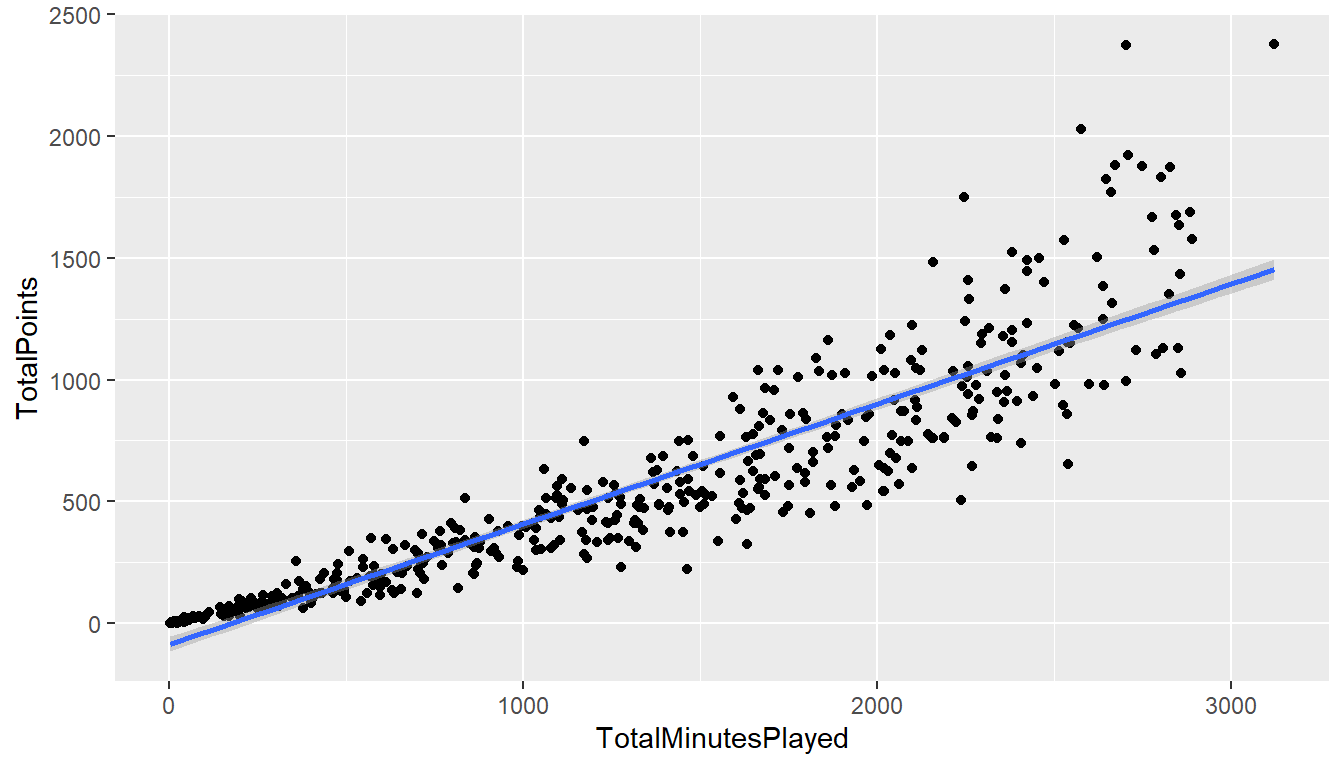
\includegraphics{DataAnalyticsWithR_files/figure-latex/linear2-1.pdf}

簡單線性迴歸分析- \texttt{glm()}

\begin{Shaded}
\begin{Highlighting}[]
\CommentTok{# formula: Y~X1+X2+...+Xn  Y:依變項 X:自變項}
\CommentTok{# data: 資料}
\KeywordTok{glm}\NormalTok{(TotalPoints~TotalMinutesPlayed,}\DataTypeTok{data =}\NormalTok{NBA1516)}
\end{Highlighting}
\end{Shaded}

\begin{verbatim}
## 
## Call:  glm(formula = TotalPoints ~ TotalMinutesPlayed, data = NBA1516)
## 
## Coefficients:
##        (Intercept)  TotalMinutesPlayed  
##           -85.9071              0.4931  
## 
## Degrees of Freedom: 475 Total (i.e. Null);  474 Residual
## Null Deviance:       99360000 
## Residual Deviance: 16720000  AIC: 6339
\end{verbatim}

TotalPoints = \texttt{0.4931} * TotalMinutesPlayed \texttt{-85.9071}

其實\texttt{glm()}是廣義線性迴歸模型 - generalized linear models (glm) -
包括了線性迴歸模型和邏輯迴歸模型 - 線性模型也可用\texttt{lm()} -
如何修改預設模型? - \texttt{family="gaussian"} 線性模型模型 -
\texttt{family="binomial"} 邏輯迴歸模型 - \texttt{family="poisson"}
卜瓦松迴歸模型

Gaussian distribution 高斯函數是\texttt{常態分布}的密度函數

Binomial distribution
二項分布是\texttt{n個獨立的是/非試驗中成功的次數}的離散機率分布

Poisson distribution \texttt{次數}分佈

\begin{itemize}
\tightlist
\item
  某一服務設施在一定時間內受到的服務請求的次數
\item
  公車站的候客人數
\item
  機器故障數
\item
  自然災害發生的次數
\item
  DNA序列的變異數\ldots{}..
\end{itemize}

\texttt{得分}與\texttt{上場分鐘數}和\texttt{兩分球出手數}的關係 -
多變量線性迴歸分析

\begin{Shaded}
\begin{Highlighting}[]
\CommentTok{# e+01: 10^1 / e-04: 10^(-4)}
\KeywordTok{glm}\NormalTok{(TotalPoints~TotalMinutesPlayed+FieldGoalsAttempted,}
    \DataTypeTok{data =}\NormalTok{NBA1516)}
\end{Highlighting}
\end{Shaded}

\begin{verbatim}
## 
## Call:  glm(formula = TotalPoints ~ TotalMinutesPlayed + FieldGoalsAttempted, 
##     data = NBA1516)
## 
## Coefficients:
##         (Intercept)   TotalMinutesPlayed  FieldGoalsAttempted  
##          -1.799e+01           -2.347e-04            1.256e+00  
## 
## Degrees of Freedom: 475 Total (i.e. Null);  473 Residual
## Null Deviance:       99360000 
## Residual Deviance: 2160000   AIC: 5367
\end{verbatim}

TotalPoints = \texttt{-0.0002347} * TotalMinutesPlayed +
\texttt{1.255794} *FieldGoalsAttempted \texttt{-17.99}

\texttt{得分}與\texttt{上場分鐘數}和\texttt{兩分球出手數}和\texttt{守備位置}的關係
- 多變量線性迴歸分析

\begin{Shaded}
\begin{Highlighting}[]
\KeywordTok{glm}\NormalTok{(TotalPoints~TotalMinutesPlayed+FieldGoalsAttempted+Position,}
    \DataTypeTok{data =}\NormalTok{NBA1516)}
\end{Highlighting}
\end{Shaded}

\begin{verbatim}
## 
## Call:  glm(formula = TotalPoints ~ TotalMinutesPlayed + FieldGoalsAttempted + 
##     Position, data = NBA1516)
## 
## Coefficients:
##         (Intercept)   TotalMinutesPlayed  FieldGoalsAttempted  
##           22.852223            -0.006537             1.275721  
##          PositionPF           PositionPG           PositionSF  
##          -39.416327           -65.034646           -38.522299  
##          PositionSG  
##          -52.175144  
## 
## Degrees of Freedom: 474 Total (i.e. Null);  468 Residual
##   (1 observation deleted due to missingness)
## Null Deviance:       99080000 
## Residual Deviance: 1975000   AIC: 5322
\end{verbatim}

\begin{Shaded}
\begin{Highlighting}[]
\CommentTok{# e+01: 10^1 / e-04: 10^(-4)}
\end{Highlighting}
\end{Shaded}

TotalPoints = \texttt{-0.0065} * TotalMinutesPlayed + \texttt{1.28}
\emph{FieldGoalsAttempted \texttt{+22.85} + \texttt{22.85} } PositionPF
+ \texttt{-65.03} * PositionPG + \texttt{-38.52} * PositionSF +
\texttt{-52.18} * PositionSG

虛擬變項 Dummy Variable

\begin{itemize}
\tightlist
\item
  PositionPF? PositionPG? PositionSF? PositionSG?
\item
  如果是控球後衛(PG),會得到\ldots{}

  \begin{itemize}
  \tightlist
  \item
    PositionPF=0
  \item
    PositionPG=1
  \item
    PositionSF=0
  \item
    PositionSG=0
  \end{itemize}
\item
  中鋒去哪了?---基準項

  \begin{itemize}
  \tightlist
  \item
    PositionPF=0
  \item
    PositionPG=0
  \item
    PositionSF=0
  \item
    PositionSG=0
  \end{itemize}
\end{itemize}

多變量線性迴歸分析

\begin{itemize}
\tightlist
\item
  假設:各變數相互獨立!
\item
  若自變項X是類別變項,需要建立\texttt{虛擬變項}
\item
  在R裡,\texttt{類別變項}請記得轉成factor,R會自動建立\texttt{虛擬變項}
\item
  用在\texttt{依變數為連續變數},\texttt{自變數為連續變數或虛擬變數}的場合
\end{itemize}

\begin{Shaded}
\begin{Highlighting}[]
\KeywordTok{class}\NormalTok{(NBA1516$Position)}
\end{Highlighting}
\end{Shaded}

\begin{verbatim}
## [1] "factor"
\end{verbatim}

\begin{Shaded}
\begin{Highlighting}[]
\KeywordTok{levels}\NormalTok{(NBA1516$Position)}
\end{Highlighting}
\end{Shaded}

\begin{verbatim}
## [1] "C"  "PF" "PG" "SF" "SG"
\end{verbatim}

用哪個計算比較準?

\begin{itemize}
\tightlist
\item
  可能不一定有適合的模型
\item
  常用的判斷準則

  \begin{itemize}
  \tightlist
  \item
    Akaike's Information Criterion (AIC)
  \item
    Bayesian Information Criterion (BIC)
  \end{itemize}
\item
  數值越小越好
\end{itemize}

用哪個計算比較準?

\begin{Shaded}
\begin{Highlighting}[]
\NormalTok{OneVar<-}\KeywordTok{glm}\NormalTok{(TotalPoints~TotalMinutesPlayed,}\DataTypeTok{data =}\NormalTok{NBA1516)}
\NormalTok{TwoVar<-}\KeywordTok{glm}\NormalTok{(TotalPoints~TotalMinutesPlayed+FieldGoalsAttempted,}
            \DataTypeTok{data =}\NormalTok{NBA1516)}
\NormalTok{ThreeVar<-}\KeywordTok{glm}\NormalTok{(TotalPoints~TotalMinutesPlayed+FieldGoalsAttempted+Position,}
              \DataTypeTok{data =}\NormalTok{NBA1516)}
\KeywordTok{c}\NormalTok{(OneVar$aic,TwoVar$aic,ThreeVar$aic)}
\end{Highlighting}
\end{Shaded}

\begin{verbatim}
## [1] 6338.913 5366.763 5321.972
\end{verbatim}

所有參數都有用嗎?

\begin{Shaded}
\begin{Highlighting}[]
\NormalTok{sum2<-}\KeywordTok{summary}\NormalTok{(TwoVar)}
\NormalTok{sum2$coefficients}
\end{Highlighting}
\end{Shaded}

\begin{verbatim}
##                          Estimate  Std. Error     t value      Pr(>|t|)
## (Intercept)         -1.798855e+01 5.659758251 -3.17832538  1.578333e-03
## TotalMinutesPlayed  -2.347183e-04 0.009474631 -0.02477334  9.802462e-01
## FieldGoalsAttempted  1.255794e+00 0.022239494 56.46682752 2.474028e-212
\end{verbatim}

所有參數都有用嗎?

\begin{Shaded}
\begin{Highlighting}[]
\NormalTok{sum3<-}\KeywordTok{summary}\NormalTok{(ThreeVar)}
\NormalTok{sum3$coefficients}
\end{Highlighting}
\end{Shaded}

\begin{verbatim}
##                          Estimate   Std. Error    t value      Pr(>|t|)
## (Intercept)          22.852222668  9.014714391  2.5349913  1.156964e-02
## TotalMinutesPlayed   -0.006536874  0.009199968 -0.7105322  4.777281e-01
## FieldGoalsAttempted   1.275721212  0.021647176 58.9324535 1.144607e-218
## PositionPF          -39.416326742  9.936541704 -3.9668053  8.425605e-05
## PositionPG          -65.034646215 10.269250388 -6.3329497  5.648565e-10
## PositionSF          -38.522298887 10.488170409 -3.6729284  2.674727e-04
## PositionSG          -52.175143670  9.985331185 -5.2251791  2.625062e-07
\end{verbatim}

\subsubsection{Logistic Regression
羅吉斯迴歸}\label{logistic-regression-}

Logistic Regression 羅吉斯迴歸

\begin{itemize}
\tightlist
\item
  用在\texttt{依變數為二元變數(非0即1)}的場合
\item
  生病/沒生病
\item
  錄取/不錄取
\item
  \texttt{family="binomial"} 邏輯迴歸模型
\end{itemize}

為什麼錄取/不錄取?

\begin{Shaded}
\begin{Highlighting}[]
\NormalTok{mydata <-}\StringTok{ }\KeywordTok{read.csv}\NormalTok{(}\StringTok{"http://www.ats.ucla.edu/stat/data/binary.csv"}\NormalTok{)}
\CommentTok{# GRE:某考試成績, GPA:在校平均成績, rank:學校聲望}
\KeywordTok{head}\NormalTok{(mydata)}
\end{Highlighting}
\end{Shaded}

\begin{verbatim}
##   admit gre  gpa rank
## 1     0 380 3.61    3
## 2     1 660 3.67    3
## 3     1 800 4.00    1
## 4     1 640 3.19    4
## 5     0 520 2.93    4
## 6     1 760 3.00    2
\end{verbatim}

Hmm\ldots{}.

\begin{Shaded}
\begin{Highlighting}[]
\NormalTok{mydata$rank <-}\StringTok{ }\KeywordTok{factor}\NormalTok{(mydata$rank)}
\NormalTok{mylogit <-}\StringTok{ }\KeywordTok{glm}\NormalTok{(admit ~}\StringTok{ }\NormalTok{gre +}\StringTok{ }\NormalTok{gpa +}\StringTok{ }\NormalTok{rank,}
               \DataTypeTok{data =} \NormalTok{mydata, }\DataTypeTok{family =} \StringTok{"binomial"}\NormalTok{)}
\NormalTok{sum<-}\KeywordTok{summary}\NormalTok{(mylogit)}
\NormalTok{sum$coefficients}
\end{Highlighting}
\end{Shaded}

\begin{verbatim}
##                 Estimate  Std. Error   z value     Pr(>|z|)
## (Intercept) -3.989979073 1.139950936 -3.500132 0.0004650273
## gre          0.002264426 0.001093998  2.069864 0.0384651284
## gpa          0.804037549 0.331819298  2.423119 0.0153878974
## rank2       -0.675442928 0.316489661 -2.134171 0.0328288188
## rank3       -1.340203916 0.345306418 -3.881202 0.0001039415
## rank4       -1.551463677 0.417831633 -3.713131 0.0002047107
\end{verbatim}

\subsection{Classification 分類}\label{classification-}

\subsubsection{Support Vector Machines
支持向量機}\label{support-vector-machines-}

\subsubsection{Decision Trees 決策樹}\label{decision-trees-}

什麼是決策樹?
在\texttt{樹狀目錄}中建立一系列分割,以建立模型。這些分割會表示成\texttt{「節點」(Node)}。每次發現輸入資料行與可預測資料行有明顯地相互關聯時,此演算法就會在模型中加入一個\texttt{節點}。演算法決定分岔的方式不同,視它預測連續資料行或分隔資料行而定。

決策樹的種類 - Classificaiton - Regression - Classification And
Regression Tree (CART)

用籃板/三分/助攻/抄截來判斷位置

\begin{Shaded}
\begin{Highlighting}[]
\KeywordTok{install.packages}\NormalTok{(}\StringTok{"rpart"}\NormalTok{)}
\end{Highlighting}
\end{Shaded}

\begin{Shaded}
\begin{Highlighting}[]
\KeywordTok{library}\NormalTok{(rpart)}
\NormalTok{DT<-}\KeywordTok{rpart}\NormalTok{(Position~Blocks+ThreesMade+Assists+Steals,}\DataTypeTok{data=}\NormalTok{NBA1516)}
\NormalTok{DT}
\end{Highlighting}
\end{Shaded}

\begin{verbatim}
## n=475 (1 observation deleted due to missingness)
## 
## node), split, n, loss, yval, (yprob)
##       * denotes terminal node
## 
##   1) root 475 364 PF (0.15 0.23 0.21 0.18 0.23)  
##     2) ThreesMade< 2.5 132  74 C (0.44 0.35 0.098 0.053 0.061)  
##       4) Blocks>=4.5 89  37 C (0.58 0.38 0.011 0.011 0.011) *
##       5) Blocks< 4.5 43  31 PF (0.14 0.28 0.28 0.14 0.16)  
##        10) Steals< 2.5 29  19 PF (0.17 0.34 0.14 0.21 0.14) *
##        11) Steals>=2.5 14   6 PG (0.071 0.14 0.57 0 0.21) *
##     3) ThreesMade>=2.5 343 242 SG (0.035 0.19 0.25 0.23 0.29)  
##       6) Assists>=170.5 96  39 PG (0.031 0.052 0.59 0.15 0.18) *
##       7) Assists< 170.5 247 163 SG (0.036 0.24 0.12 0.26 0.34)  
##        14) Blocks>=20.5 80  42 PF (0.062 0.48 0 0.26 0.2)  
##          28) Steals< 59.5 58  21 PF (0.069 0.64 0 0.14 0.16) *
##          29) Steals>=59.5 22   9 SF (0.045 0.045 0 0.59 0.32) *
##        15) Blocks< 20.5 167  99 SG (0.024 0.13 0.17 0.26 0.41)  
##          30) Assists< 81.5 110  68 SG (0.027 0.18 0.091 0.32 0.38)  
##            60) Blocks>=4.5 63  39 SF (0.032 0.29 0.016 0.38 0.29)  
##             120) ThreesMade< 13.5 19   9 PF (0.11 0.53 0 0.26 0.11) *
##             121) ThreesMade>=13.5 44  25 SF (0 0.18 0.023 0.43 0.36)  
##               242) Blocks< 9.5 17   7 SF (0 0.18 0.059 0.59 0.18) *
##               243) Blocks>=9.5 27  14 SG (0 0.19 0 0.33 0.48) *
##            61) Blocks< 4.5 47  23 SG (0.021 0.043 0.19 0.23 0.51) *
##          31) Assists>=81.5 57  31 SG (0.018 0.035 0.33 0.16 0.46)  
##            62) ThreesMade< 37 17   5 PG (0 0.12 0.71 0.059 0.12) *
##            63) ThreesMade>=37 40  16 SG (0.025 0 0.17 0.2 0.6) *
\end{verbatim}

\begin{Shaded}
\begin{Highlighting}[]
\CommentTok{#控球後衛(PG)、得分後衛(SG)、小前鋒(SF)、大前鋒(PF)和中鋒(C)}
\end{Highlighting}
\end{Shaded}

用籃板/三分/助攻/抄截來判斷位置

\begin{Shaded}
\begin{Highlighting}[]
\KeywordTok{par}\NormalTok{(}\DataTypeTok{mfrow=}\KeywordTok{c}\NormalTok{(}\DecValTok{1}\NormalTok{,}\DecValTok{1}\NormalTok{), }\DataTypeTok{mar =} \KeywordTok{rep}\NormalTok{(}\DecValTok{1}\NormalTok{,}\DecValTok{4}\NormalTok{)) }\CommentTok{#下,左,上,右}
\KeywordTok{plot}\NormalTok{(DT)}
\KeywordTok{text}\NormalTok{(DT, }\DataTypeTok{use.n=}\NormalTok{F, }\DataTypeTok{all=}\NormalTok{F, }\DataTypeTok{cex=}\DecValTok{1}\NormalTok{)}
\end{Highlighting}
\end{Shaded}

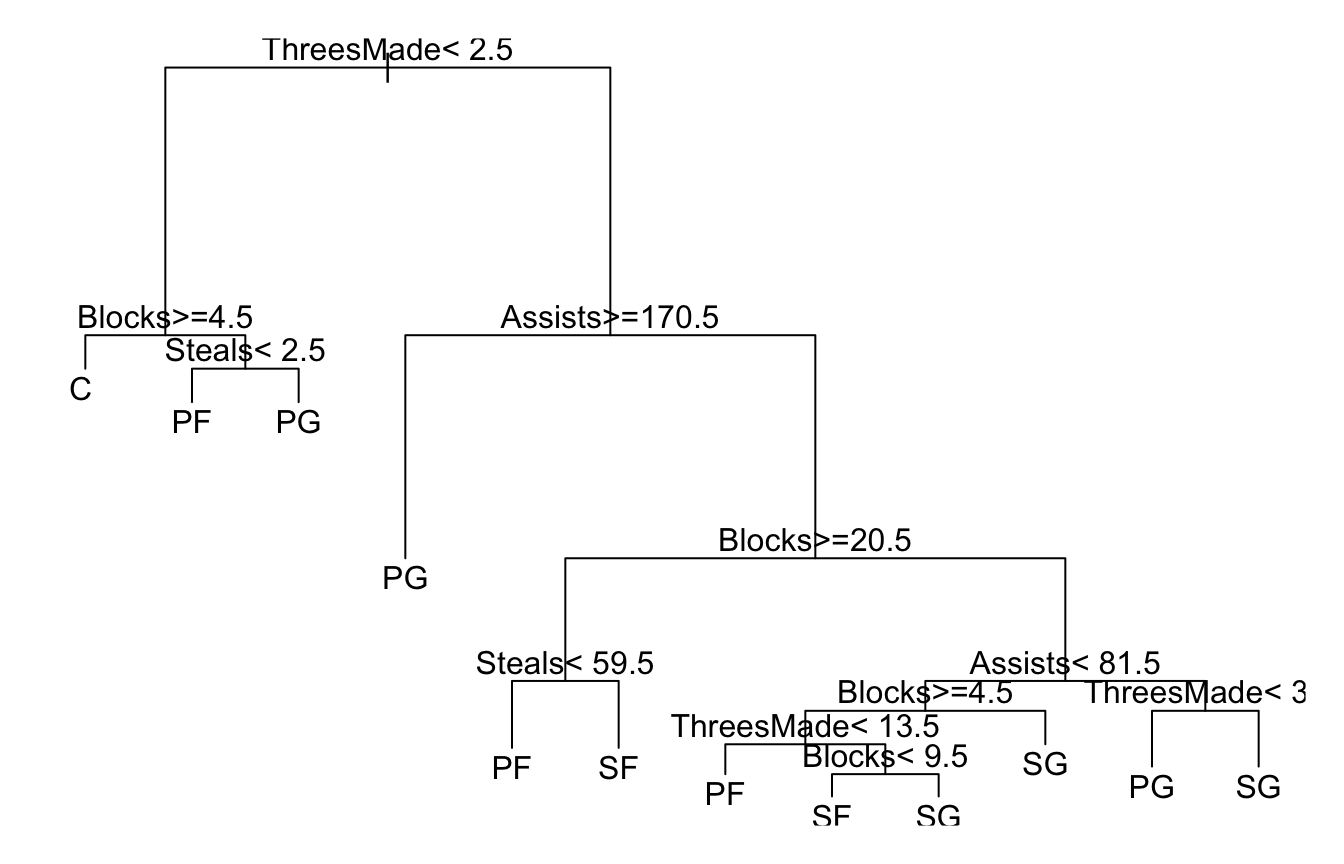
\includegraphics{DataAnalyticsWithR_files/figure-latex/rpart3-1.pdf}

\begin{Shaded}
\begin{Highlighting}[]
\CommentTok{#控球後衛(PG)、得分後衛(SG)、小前鋒(SF)、大前鋒(PF)和中鋒(C)}
\end{Highlighting}
\end{Shaded}

用籃板/三分/助攻/抄截來判斷位置
預設的\texttt{plot()}真的太難用,改用\texttt{rpart.plot}
package裡面的\texttt{prp()}

\begin{Shaded}
\begin{Highlighting}[]
\KeywordTok{install.packages}\NormalTok{(}\StringTok{"rpart.plot"}\NormalTok{)}
\end{Highlighting}
\end{Shaded}

\begin{Shaded}
\begin{Highlighting}[]
\KeywordTok{library}\NormalTok{(rpart.plot)}
\KeywordTok{prp}\NormalTok{(DT)                 }\CommentTok{# Will plot the tree}
\end{Highlighting}
\end{Shaded}

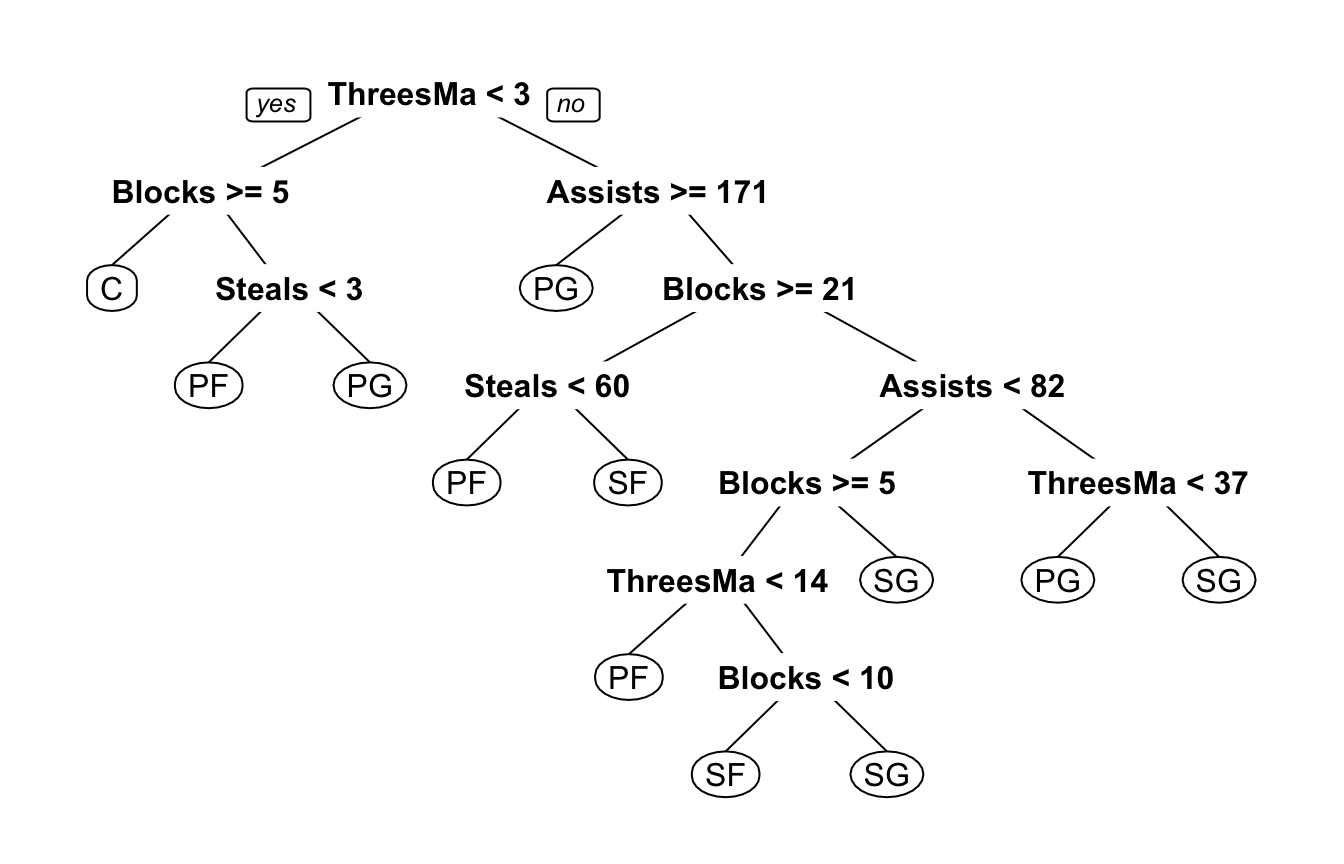
\includegraphics{DataAnalyticsWithR_files/figure-latex/rpart4-1.pdf}

用籃板/三分/助攻/抄截來判斷位置

\begin{Shaded}
\begin{Highlighting}[]
\KeywordTok{prp}\NormalTok{(DT)}
\end{Highlighting}
\end{Shaded}

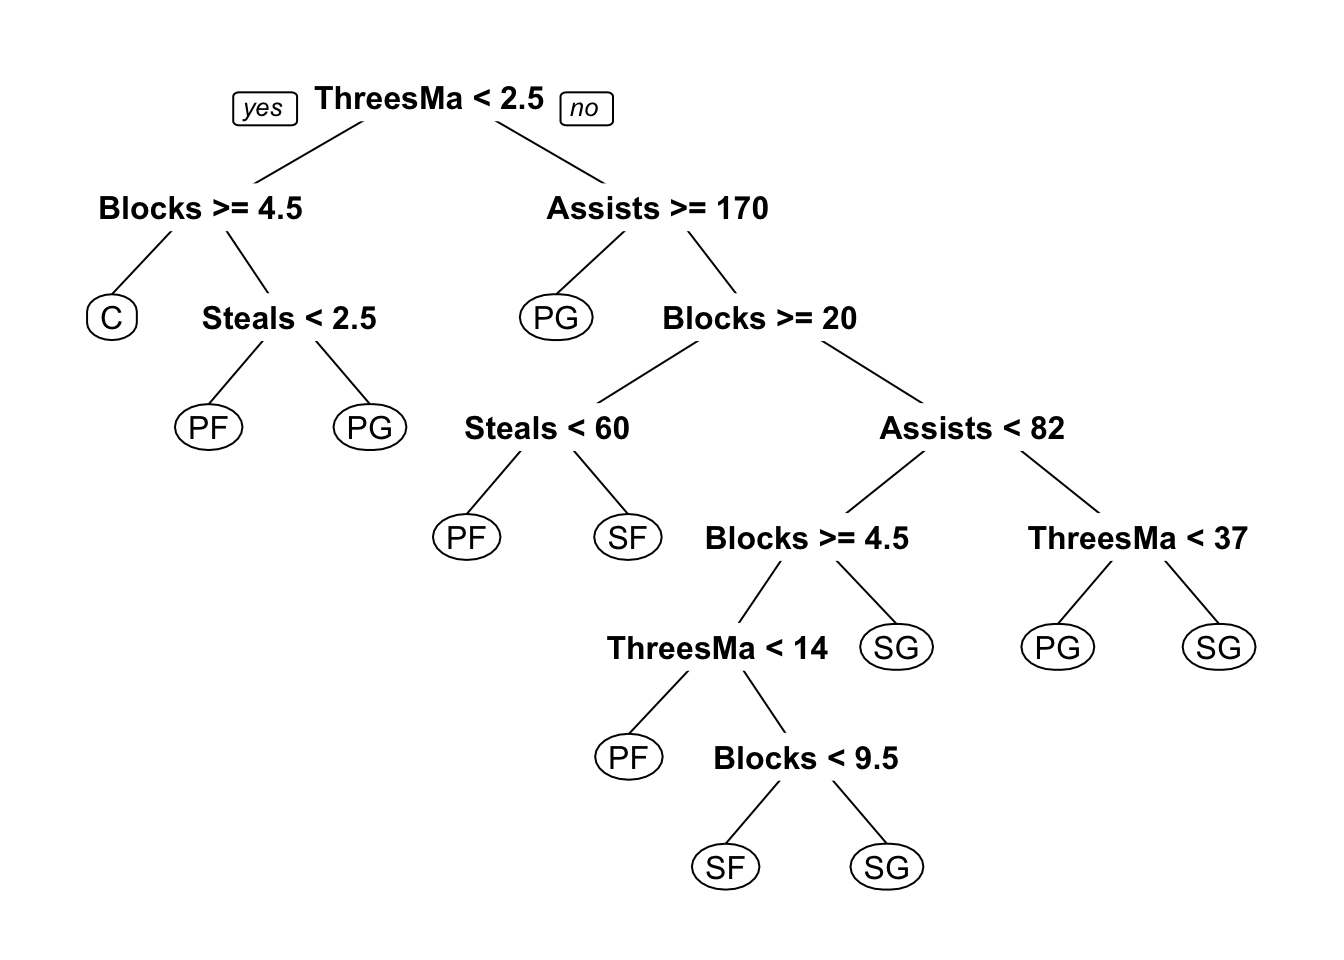
\includegraphics{DataAnalyticsWithR_files/figure-latex/rpart5-1.pdf}

決策樹演算法怎麼決定\texttt{節點} - Gini impurity - Information gain -
Variance reduction

\ldots{}有機會再說吧\ldots{}\ldots{}

\subsubsection{Neural Networks 神經網路}\label{neural-networks-}

\subsubsection{K-Nearest Neighbor}\label{k-nearest-neighbor}

\section{非監督式學習}

\subsection{Clustering 分群}\label{clustering-}

如何找到相似的物件/事件?

Clustering organizes things that are \texttt{close} into groups

\begin{itemize}
\tightlist
\item
  How do we define close?
\item
  How do we group things?
\item
  How do we visualize the grouping?
\item
  How do we interpret the grouping?
\end{itemize}

\subsubsection{Hierarchical clustering
階層式分群}\label{hierarchical-clustering-}

\begin{itemize}
\tightlist
\item
  An agglomerative approach

  \begin{itemize}
  \tightlist
  \item
    Find closest two things
  \item
    Put them together
  \item
    Find next closest
  \end{itemize}
\item
  Requires

  \begin{itemize}
  \tightlist
  \item
    A defined distance
  \item
    A merging approach
  \end{itemize}
\item
  Produces

  \begin{itemize}
  \tightlist
  \item
    A tree showing how close things are to each other
  \end{itemize}
\end{itemize}

Hierarchical clustering

\begin{itemize}
\tightlist
\item
  An agglomerative approach

  \begin{itemize}
  \tightlist
  \item
    Find closest two things
  \item
    Put them together
  \item
    Find next closest
  \end{itemize}
\item
  Requires

  \begin{itemize}
  \tightlist
  \item
    \texttt{A\ defined\ distance}
  \item
    A merging approach
  \end{itemize}
\item
  Produces

  \begin{itemize}
  \tightlist
  \item
    A tree showing how close things are to each other
  \end{itemize}
\end{itemize}

How do we define close? \texttt{distance}

\begin{itemize}
\tightlist
\item
  Most important step

  \begin{itemize}
  \tightlist
  \item
    Garbage in -\textgreater{} garbage out
  \end{itemize}
\item
  Distance or similarity

  \begin{itemize}
  \tightlist
  \item
    Continuous - euclidean distance
  \item
    Continuous - correlation similarity
  \item
    Binary - manhattan distance
  \end{itemize}
\item
  Pick a distance/similarity that makes sense for your problem
\end{itemize}

Example distances - Euclidean

\[\sqrt{(A_1-A_2)^2 + (B_1-B_2)^2 + \ldots + (Z_1-Z_2)^2}\]

Example distances - Manhattan

\[|A_1-A_2| + |B_1-B_2| + \ldots + |Z_1-Z_2|\]

Green line: Euclidean, Blue line: Manhattan

Hierarchical clustering

\begin{itemize}
\tightlist
\item
  An agglomerative approach

  \begin{itemize}
  \tightlist
  \item
    Find closest two things
  \item
    Put them together
  \item
    Find next closest
  \end{itemize}
\item
  Requires

  \begin{itemize}
  \tightlist
  \item
    A defined distance
  \item
    \texttt{A\ merging\ approach}
  \end{itemize}
\item
  Produces

  \begin{itemize}
  \tightlist
  \item
    A tree showing how close things are to each other
  \end{itemize}
\end{itemize}

Merging apporach - Agglomerative 聚合 - Single-linkage:取最小值 -
Complete-linkage:取最大值 - Average-linkage:取平均值

Hierarchical clustering - hp vs.~mpg
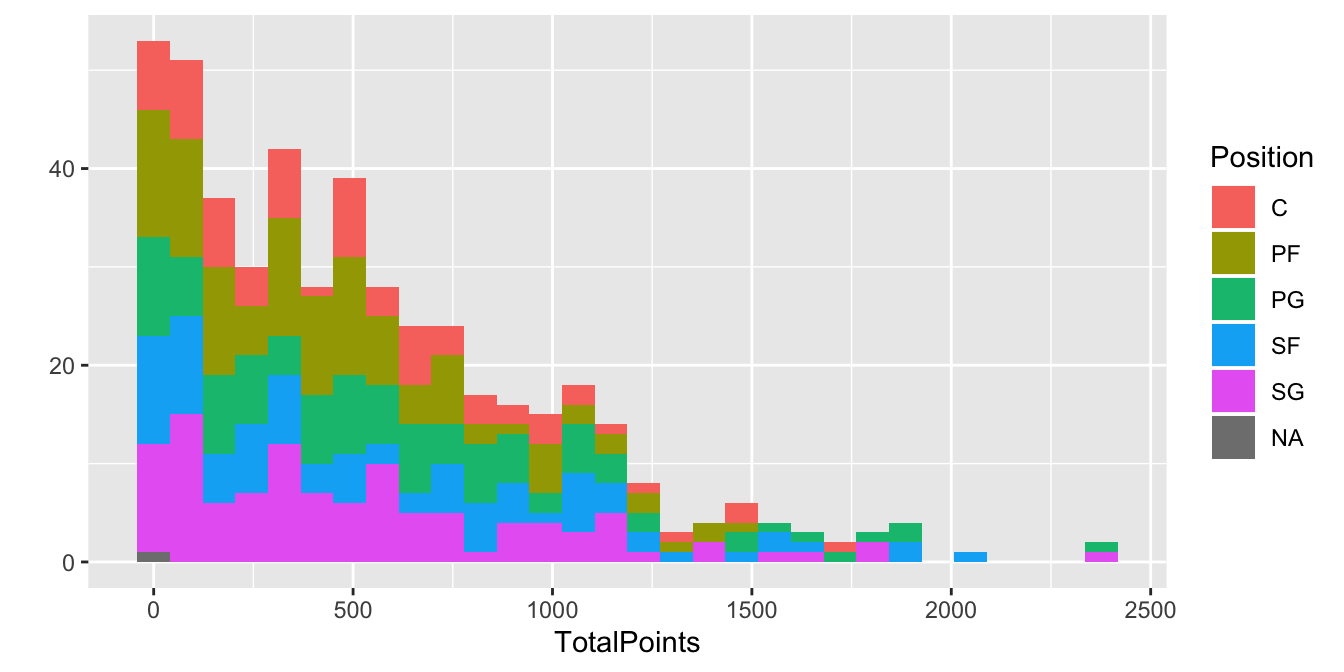
\includegraphics{DataAnalyticsWithR_files/figure-latex/unnamed-chunk-1-1.pdf}

Hierarchical clustering - \#1

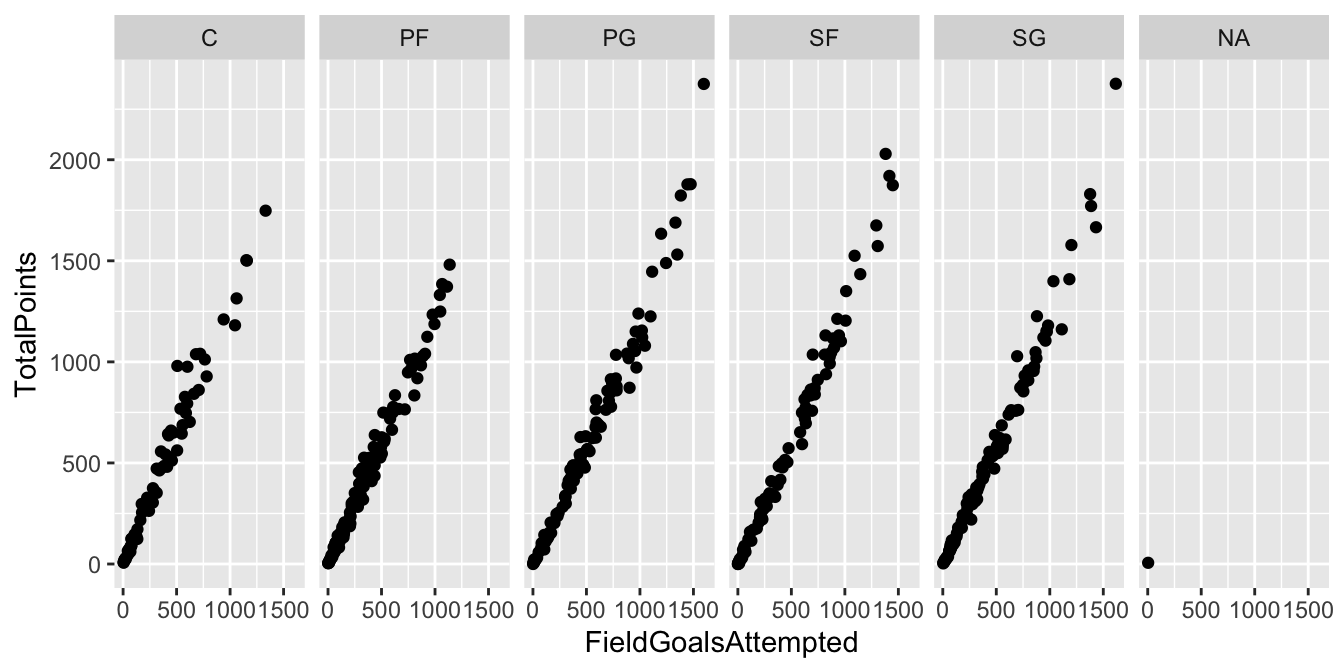
\includegraphics{DataAnalyticsWithR_files/figure-latex/unnamed-chunk-2-1.pdf}

Hierarchical clustering - \#2
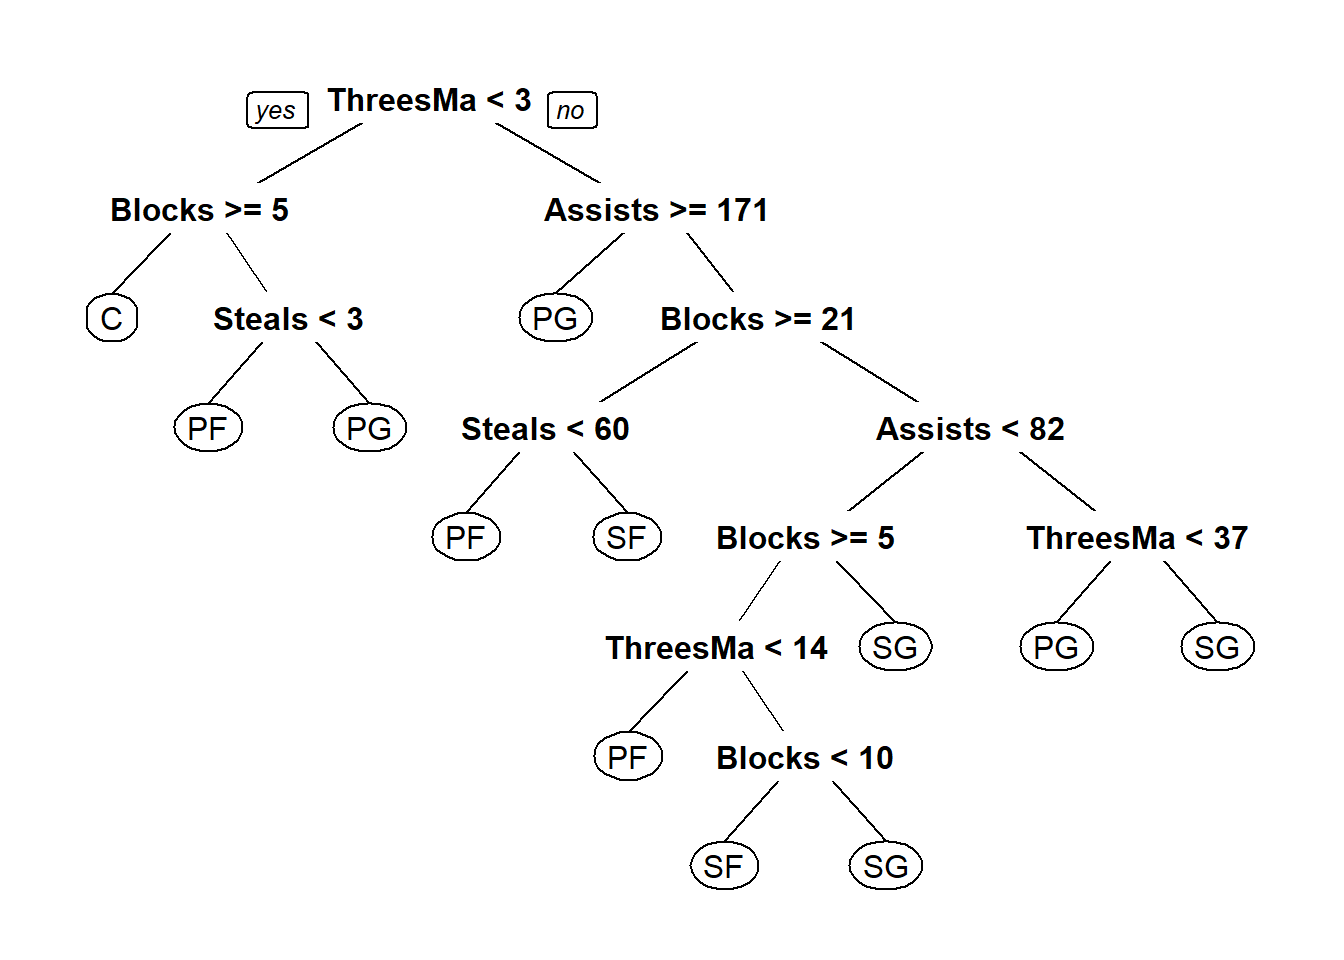
\includegraphics{DataAnalyticsWithR_files/figure-latex/unnamed-chunk-3-1.pdf}

Hierarchical clustering - \#3

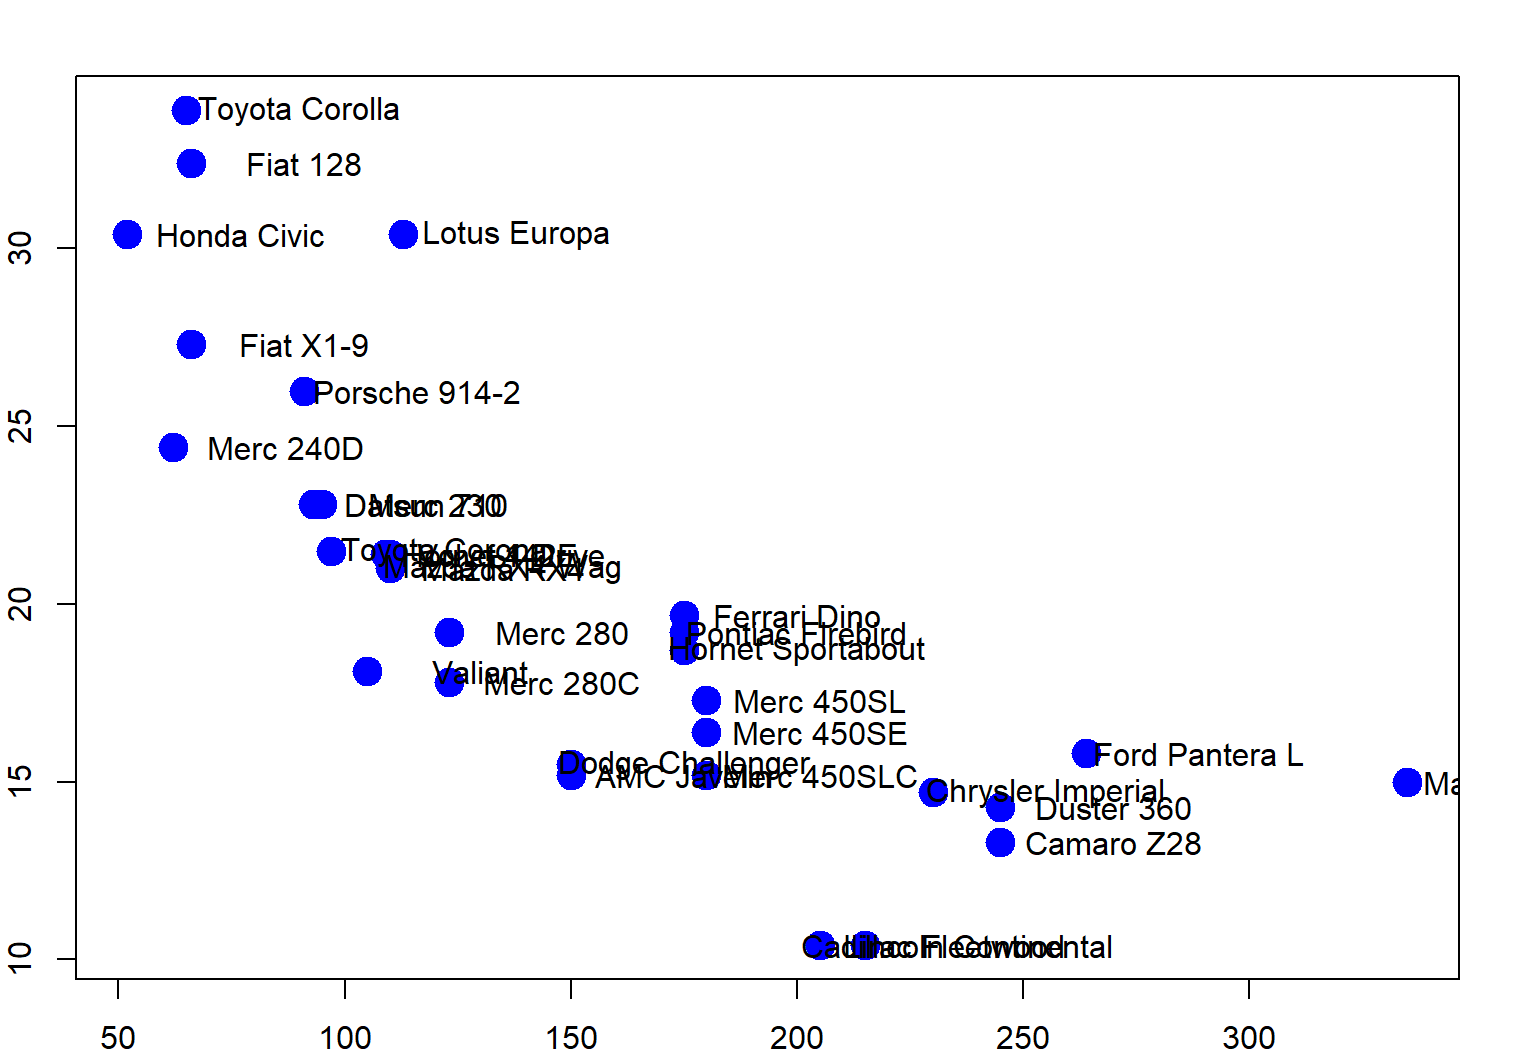
\includegraphics{DataAnalyticsWithR_files/figure-latex/unnamed-chunk-4-1.pdf}

Hierarchical clustering

\begin{itemize}
\tightlist
\item
  An agglomerative approach

  \begin{itemize}
  \tightlist
  \item
    Find closest two things
  \item
    Put them together
  \item
    Find next closest
  \end{itemize}
\item
  \texttt{Requires}

  \begin{itemize}
  \tightlist
  \item
    A defined distance
  \item
    A merging approach
  \end{itemize}
\item
  Produces

  \begin{itemize}
  \tightlist
  \item
    A tree showing how close things are to each other
  \end{itemize}
\end{itemize}

Hierarchical Clustering -dist()
用\texttt{dist()}函數計算距離,使用method=``''設定計算距離的依據

\begin{Shaded}
\begin{Highlighting}[]
\NormalTok{mtcars.mxs<-}\KeywordTok{as.matrix}\NormalTok{(mtcars)}
\NormalTok{d<-}\KeywordTok{dist}\NormalTok{(mtcars.mxs) }\CommentTok{#預設為euclidean}
\NormalTok{d}
\end{Highlighting}
\end{Shaded}

\begin{verbatim}
##                       Mazda RX4 Mazda RX4 Wag  Datsun 710 Hornet 4 Drive
## Mazda RX4 Wag         0.6153251                                         
## Datsun 710           54.9086059    54.8915169                           
## Hornet 4 Drive       98.1125212    98.0958939 150.9935191               
## Hornet Sportabout   210.3374396   210.3358546 265.0831615    121.0297564
## Valiant              65.4717710    65.4392224 117.7547018     33.5508692
## Duster 360          241.4076490   241.4088680 294.4790230    169.4299647
## Merc 240D            50.1532711    50.1146059  49.6584796    121.2739722
## Merc 230             25.4683117    25.3284509  33.1803843    118.2433145
## Merc 280             15.3641921    15.2956865  66.9363534     91.4224033
## Merc 280C            15.6724727    15.5837744  67.0261397     91.4612914
## Merc 450SE          135.4307018   135.4254826 189.1954941     72.4964325
## Merc 450SL          135.4014424   135.3960351 189.1631745     72.4313532
## Merc 450SLC         135.4794674   135.4723157 189.2345426     72.5718466
## Cadillac Fleetwood  326.3395903   326.3355070 381.0926242    234.4403876
## Lincoln Continental 318.0469808   318.0429333 372.8012090    227.9726091
## Chrysler Imperial   304.7203408   304.7169175 359.3014906    218.1548299
## Fiat 128             93.2679950    93.2530993  40.9933763    184.9689734
## Honda Civic         102.8307567   102.8238713  52.7704607    191.5518700
## Toyota Corolla      100.6040368   100.5887588  47.6535017    192.6714187
## Toyota Corona        42.3075233    42.2659224  12.9654743    138.5304725
## Dodge Challenger    163.1150750   163.1134210 217.7795805     72.4403915
## AMC Javelin         149.6047203   149.6014522 204.3188913     61.3601899
## Camaro Z28          233.2228758   233.2248748 286.0049209    163.6632641
## Pontiac Firebird    248.6780270   248.6762035 303.3583889    156.2240346
## Fiat X1-9            92.5048389    92.4940020  39.8815148    184.4471198
## Porsche 914-2        44.4033659    44.4073589  13.1357109    139.1579524
## Lotus Europa         65.7328377    65.7362635  25.0948550    163.2367437
## Ford Pantera L      245.4247064   245.4293785 297.2940489    180.1140339
## Ferrari Dino         66.7661029    66.7764167  90.2415509    130.5523007
## Maserati Bora       265.6454248   265.6491465 309.7718171    229.3419352
## Volvo 142E           39.1894029    39.1626037  20.6939436    137.0363299
##                     Hornet Sportabout     Valiant  Duster 360   Merc 240D
## Mazda RX4 Wag                                                            
## Datsun 710                                                               
## Hornet 4 Drive                                                           
## Hornet Sportabout                                                        
## Valiant                   152.1241352                                    
## Duster 360                 70.1767262 194.6094525                        
## Merc 240D                 241.5069657  89.5911056 281.2962502            
## Merc 230                  233.4924012  85.0079649 265.8823313  33.6873047
## Merc 280                  199.3344960  60.2909811 227.8998521  64.7754228
## Merc 280C                 199.3406564  60.2655656 227.8813169  64.8898713
## Merc 450SE                 84.3888482  90.6970264 106.4084264 175.1620073
## Merc 450SL                 84.3683999  90.6769728 106.4320572 175.1189767
## Merc 450SLC                84.4332423  90.7092989 106.4010305 175.2118218
## Cadillac Fleetwood        116.2804201 266.6280942 119.0239068 355.6627498
## Lincoln Continental       108.0624299 259.6304391 104.5112999 348.9901277
## Chrysler Imperial          97.2049146 248.7713290  81.4297699 338.1959373
## Fiat 128                  302.0377212 152.1153263 333.9792070  68.6105903
## Honda Civic               310.0324645 158.9615769 344.0518316  72.0014488
## Toyota Corolla            309.5581776 159.8302995 341.0218232  76.2806458
## Toyota Corona             252.3331988 105.2876428 282.0508820  44.0850975
## Dodge Challenger           48.9838851 103.4310693 103.9023864 192.8617917
## AMC Javelin                61.4274240  91.0444349 110.3084921 180.5479760
## Camaro Z28                 70.9665308 187.8463771  10.0761203 273.8367985
## Pontiac Firebird           40.0052475 188.5272116  80.8057339 277.4606884
## Fiat X1-9                 301.5669483 151.4379425 333.4843231  67.9163981
## Porsche 914-2             254.1452553 106.0585767 285.1986201  39.4469276
## Lotus Europa              272.3582423 130.8248192 296.4572287  72.8971106
## Ford Pantera L             89.5934049 203.0177926  21.2655990 287.5238795
## Ferrari Dino              215.0673853 106.5694802 226.2036333 113.3023005
## Maserati Bora             170.7094473 242.4393015 107.7224977 313.8633093
## Volvo 142E                248.0063378 104.1863681 275.1353516  53.6823481
##                        Merc 230    Merc 280   Merc 280C  Merc 450SE
## Mazda RX4 Wag                                                      
## Datsun 710                                                         
## Hornet 4 Drive                                                     
## Hornet Sportabout                                                  
## Valiant                                                            
## Duster 360                                                         
## Merc 240D                                                          
## Merc 230                                                           
## Merc 280             39.2994160                                    
## Merc 280C            39.3868519   1.5231546                        
## Merc 450SE          159.8179555 122.3642489 122.3461050            
## Merc 450SL          159.7760899 122.3443771 122.3355492   0.9826495
## Merc 450SLC         159.8495837 122.3934970 122.3586862   1.3726252
## Cadillac Fleetwood  349.2832611 315.3904859 315.3557081 197.8842803
## Lincoln Continental 341.3154316 306.6760719 306.6406187 187.5997191
## Chrysler Imperial   328.4335161 292.7146896 292.6989332 171.6600758
## Fiat 128             69.3127910 106.5053149 106.6829794 228.3247948
## Honda Civic          78.5387212 116.7280991 116.8711475 238.0141824
## Toyota Corolla       76.7731674 113.6290721 113.8118009 235.5183809
## Toyota Corona        21.0962017  54.3641713  54.4258314 176.6020527
## Dodge Challenger    185.8331870 152.8929263 152.8722437  51.8008639
## AMC Javelin         172.5312555 139.1457974 139.1181977  41.2080044
## Camaro Z28          257.7469734 219.5520854 219.5276434  98.7203049
## Pontiac Firebird    271.3871978 238.1726099 238.1806292 124.3368538
## Fiat X1-9            68.5564864 105.7412910 105.8560373 227.7627676
## Porsche 914-2        22.1180967  57.6458160  57.8473863 179.5034108
## Lotus Europa         50.1094030  74.1443580  74.3824296 193.3074449
## Ford Pantera L      269.9772035 231.4081306 231.4024263 112.8181834
## Ferrari Dino         80.6550953  56.8365103  56.8987601 131.0272205
## Maserati Bora       288.8755628 250.5874125 250.5774357 157.1633256
## Volvo 142E           24.6913548  48.8053450  48.8884618 170.4500681
##                      Merc 450SL Merc 450SLC Cadillac Fleetwood
## Mazda RX4 Wag                                                 
## Datsun 710                                                    
## Hornet 4 Drive                                                
## Hornet Sportabout                                             
## Valiant                                                       
## Duster 360                                                    
## Merc 240D                                                     
## Merc 230                                                      
## Merc 280                                                      
## Merc 280C                                                     
## Merc 450SE                                                    
## Merc 450SL                                                    
## Merc 450SLC           2.1383405                               
## Cadillac Fleetwood  197.9154476 197.8526242                   
## Lincoln Continental 187.6330806 187.5671081         15.6224446
## Chrysler Imperial   171.6743028 171.6557637         40.8399636
## Fiat 128            228.2592340 228.4051825        417.7687579
## Honda Civic         237.9588183 238.0828999        425.3271621
## Toyota Corolla      235.4481971 235.6024098        425.3446517
## Toyota Corona       176.5727477 176.6305359        368.3195488
## Dodge Challenger     51.8242520  51.8012606        163.6314881
## AMC Javelin          41.2411618  41.1929050        176.8610896
## Camaro Z28           98.7566899  98.7035830        128.4587210
## Pontiac Firebird    124.3204160 124.3726128         78.5385347
## Fiat X1-9           227.7173075 227.8176554        417.2490481
## Porsche 914-2       179.4550855 179.5720446        370.0956775
## Lotus Europa        193.2407697 193.3969216        388.5350012
## Ford Pantera L      112.8296774 112.8332602        134.8119464
## Ferrari Dino        131.0077635 131.0704490        328.5441628
## Maserati Bora       157.1768956 157.1683970        214.9366858
## Volvo 142E          170.4225164 170.4843735        364.1000930
##                     Lincoln Continental Chrysler Imperial    Fiat 128
## Mazda RX4 Wag                                                        
## Datsun 710                                                           
## Hornet 4 Drive                                                       
## Hornet Sportabout                                                    
## Valiant                                                              
## Duster 360                                                           
## Merc 240D                                                            
## Merc 230                                                             
## Merc 280                                                             
## Merc 280C                                                            
## Merc 450SE                                                           
## Merc 450SL                                                           
## Merc 450SLC                                                          
## Cadillac Fleetwood                                                   
## Lincoln Continental                                                  
## Chrysler Imperial            25.3714237                              
## Fiat 128                    410.0206984       397.2276375            
## Honda Civic                 417.9679574       405.8152201  14.5590942
## Toyota Corolla              417.5429986       404.6335386   7.8324789
## Toyota Corona               360.0267515       346.5724649  52.8798281
## Dodge Challenger            156.2805020       145.9194779 254.2367888
## AMC Javelin                 169.0925457       157.8097554 241.1203621
## Camaro Z28                  114.0932078        91.2880886 325.6636235
## Pontiac Firebird             72.6947903        68.2030747 339.5857659
## Fiat X1-9                   409.4998363       396.7597522   5.1473415
## Porsche 914-2               362.0145494       348.8466861  49.0644372
## Lotus Europa                379.4716659       364.5994326  49.9112509
## Ford Pantera L              119.7236456        95.3805385 337.1639236
## Ferrari Dino                317.7063117       300.1640703 128.3950054
## Maserati Bora               199.3420611       174.2936864 349.5338830
## Volvo 142E                  355.4009443       341.2896659  61.3301247
##                     Honda Civic Toyota Corolla Toyota Corona
## Mazda RX4 Wag                                               
## Datsun 710                                                  
## Hornet 4 Drive                                              
## Hornet Sportabout                                           
## Valiant                                                     
## Duster 360                                                  
## Merc 240D                                                   
## Merc 230                                                    
## Merc 280                                                    
## Merc 280C                                                   
## Merc 450SE                                                  
## Merc 450SL                                                  
## Merc 450SLC                                                 
## Cadillac Fleetwood                                          
## Lincoln Continental                                         
## Chrysler Imperial                                           
## Fiat 128                                                    
## Honda Civic                                                 
## Toyota Corolla       14.3480626                             
## Toyota Corona        63.8985563     59.8451285              
## Dodge Challenger    261.8498815    261.8345312   205.0347927
## AMC Javelin         248.9636504    248.6917065   191.5580526
## Camaro Z28          335.8883188    332.6589699   273.6316895
## Pontiac Firebird    347.0655360    347.1667643   290.6240706
## Fiat X1-9            14.7807070     10.3922856    51.8411748
## Porsche 914-2        59.4588768     56.3243031     8.6535903
## Lotus Europa         64.0495153     53.8846563    31.2536926
## Ford Pantera L      347.8337714    343.9920962   285.1287911
## Ferrari Dino        141.7044478    133.4707617    82.2355734
## Maserati Bora       362.1620777    355.2601619   299.1865216
## Volvo 142E           73.3766041     67.7189421    12.2505275
##                     Dodge Challenger AMC Javelin  Camaro Z28
## Mazda RX4 Wag                                               
## Datsun 710                                                  
## Hornet 4 Drive                                              
## Hornet Sportabout                                           
## Valiant                                                     
## Duster 360                                                  
## Merc 240D                                                   
## Merc 230                                                    
## Merc 280                                                    
## Merc 280C                                                   
## Merc 450SE                                                  
## Merc 450SL                                                  
## Merc 450SLC                                                 
## Cadillac Fleetwood                                          
## Lincoln Continental                                         
## Chrysler Imperial                                           
## Fiat 128                                                    
## Honda Civic                                                 
## Toyota Corolla                                              
## Toyota Corona                                               
## Dodge Challenger                                            
## AMC Javelin               14.0154995                        
## Camaro Z28               100.3046106 105.6062618            
## Pontiac Firebird          85.8075196  99.2836114  86.2665759
## Fiat X1-9                253.6624046 240.5266823 325.1490914
## Porsche 914-2            206.6452569 193.3080584 276.8924414
## Lotus Europa             226.5004836 212.7568765 287.6179004
## Ford Pantera L           118.7516779 123.3832044  19.3589023
## Ferrari Dino             174.9280395 161.1060307 216.7489910
## Maserati Bora            185.9059273 185.1553411 102.5946154
## Volvo 142E               201.3682522 187.6978440 266.5277736
##                     Pontiac Firebird   Fiat X1-9 Porsche 914-2
## Mazda RX4 Wag                                                 
## Datsun 710                                                    
## Hornet 4 Drive                                                
## Hornet Sportabout                                             
## Valiant                                                       
## Duster 360                                                    
## Merc 240D                                                     
## Merc 230                                                      
## Merc 280                                                      
## Merc 280C                                                     
## Merc 450SE                                                    
## Merc 450SL                                                    
## Merc 450SLC                                                   
## Cadillac Fleetwood                                            
## Lincoln Continental                                           
## Chrysler Imperial                                             
## Fiat 128                                                      
## Honda Civic                                                   
## Toyota Corolla                                                
## Toyota Corona                                                 
## Dodge Challenger                                              
## AMC Javelin                                                   
## Camaro Z28                                                    
## Pontiac Firebird                                              
## Fiat X1-9                339.1396182                          
## Porsche 914-2            292.1646488  48.3775209              
## Lotus Europa             311.3862342  49.8406880    33.7678653
## Ford Pantera L           101.7389686 336.7018783   288.5852993
## Ferrari Dino             255.0570519 127.8210813    87.9105966
## Maserati Bora            188.3240020 349.1199576   303.9222549
## Volvo 142E               286.7497823  60.4120429    18.7555858
##                     Lotus Europa Ford Pantera L Ferrari Dino Maserati Bora
## Mazda RX4 Wag                                                             
## Datsun 710                                                                
## Hornet 4 Drive                                                            
## Hornet Sportabout                                                         
## Valiant                                                                   
## Duster 360                                                                
## Merc 240D                                                                 
## Merc 230                                                                  
## Merc 280                                                                  
## Merc 280C                                                                 
## Merc 450SE                                                                
## Merc 450SL                                                                
## Merc 450SLC                                                               
## Cadillac Fleetwood                                                        
## Lincoln Continental                                                       
## Chrysler Imperial                                                         
## Fiat 128                                                                  
## Honda Civic                                                               
## Toyota Corolla                                                            
## Toyota Corona                                                             
## Dodge Challenger                                                          
## AMC Javelin                                                               
## Camaro Z28                                                                
## Pontiac Firebird                                                          
## Fiat X1-9                                                                 
## Porsche 914-2                                                             
## Lotus Europa                                                              
## Ford Pantera L       297.5376920                                          
## Ferrari Dino          80.4553451    224.4587490                           
## Maserati Bora        303.2796468     86.9383253  223.5342175              
## Volvo 142E            27.8104457    277.4803312   70.4751034   289.1157363
\end{verbatim}

Hierarchical Clustering -dist()
用\texttt{dist()}函數計算距離,使用method=``''設定計算距離的依據,可用方法包括:
``euclidean'', ``maximum'', ``manhattan'', ``canberra'', ``binary'' or
``minkowski''

\begin{Shaded}
\begin{Highlighting}[]
\NormalTok{d<-}\KeywordTok{dist}\NormalTok{(mtcars.mxs, }\DataTypeTok{method=}\StringTok{"manhattan"}\NormalTok{) }\CommentTok{#計算manhattan距離}
\NormalTok{d}
\end{Highlighting}
\end{Shaded}

\begin{verbatim}
##                     Mazda RX4 Mazda RX4 Wag Datsun 710 Hornet 4 Drive
## Mazda RX4 Wag           0.815                                        
## Datsun 710             79.300        78.995                          
## Hornet 4 Drive        108.795       107.980    174.895               
## Hornet Sportabout     275.430       274.615    349.510        176.415
## Valiant                84.640        83.825    141.540         42.645
## Duster 360            347.960       348.265    427.160        254.185
## Merc 240D              75.020        74.205     75.720        167.495
## Merc 230               48.990        48.175     41.990        141.965
## Merc 280               27.080        26.265    100.700        111.805
## Merc 280C              29.080        28.265    102.080        112.605
## Merc 450SE            198.620       197.805    273.940        100.705
## Merc 450SL            197.580       196.765    272.500         99.265
## Merc 450SLC           200.130       199.315    274.250        101.015
## Cadillac Fleetwood    426.720       425.905    502.880        329.645
## Lincoln Continental   424.664       423.849    501.144        327.909
## Chrysler Imperial     414.655       413.840    491.935        319.000
## Fiat 128              146.310       146.005     67.110        240.345
## Honda Civic           160.795       160.490     83.775        258.670
## Toyota Corolla        157.345       157.040     78.145        251.380
## Toyota Corona          65.305        65.000     21.095        154.940
## Dodge Challenger      211.950       211.435    286.330        113.095
## AMC Javelin           198.205       197.390    271.725         98.630
## Camaro Z28            339.140       339.445    418.340        246.405
## Pontiac Firebird      315.435       314.620    389.455        216.220
## Fiat X1-9             140.605       140.300     61.405        235.720
## Porsche 914-2          69.950        70.285     23.170        173.465
## Lotus Europa           84.977        84.912     45.097        185.832
## Ford Pantera L        356.030       356.335    435.330        267.725
## Ferrari Dino           85.690        86.205    134.890        193.625
## Maserati Bora         382.170       382.475    461.370        293.055
## Volvo 142E             47.910        47.285     32.130        145.305
##                     Hornet Sportabout Valiant Duster 360 Merc 240D
## Mazda RX4 Wag                                                     
## Datsun 710                                                        
## Hornet 4 Drive                                                    
## Hornet Sportabout                                                 
## Valiant                       213.210                             
## Duster 360                     77.770 289.740                     
## Merc 240D                     341.770 133.020    419.420          
## Merc 230                      316.240 107.050    393.890    43.670
## Merc 280                      252.950  83.600    326.600    93.280
## Merc 280C                     253.950  82.200    325.800    94.080
## Merc 450SE                     93.590 136.240    154.500   266.200
## Merc 450SL                     92.550 134.800    155.260   264.760
## Merc 450SLC                    95.100 136.550    153.610   266.510
## Cadillac Fleetwood            155.290 364.900    160.000   495.140
## Lincoln Continental           153.234 363.304    137.944   493.404
## Chrysler Imperial             143.385 354.555     98.775   484.195
## Fiat 128                      416.620 206.930    494.270    83.910
## Honda Civic                   431.105 225.315    508.755    92.295
## Toyota Corolla                427.655 217.105    505.305    92.085
## Toyota Corona                 331.215 120.445    408.865    67.245
## Dodge Challenger               70.820 148.010    141.730   278.590
## AMC Javelin                    84.785 134.235    155.555   263.985
## Camaro Z28                     89.990 281.960     12.220   410.680
## Pontiac Firebird               41.005 253.975    118.515   381.715
## Fiat X1-9                     410.915 202.365    488.565    79.345
## Porsche 914-2                 340.900 140.110    417.910    65.090
## Lotus Europa                  349.267 162.477    426.677   115.457
## Ford Pantera L                109.760 303.770     35.250   429.950
## Ferrari Dino                  227.660 166.870    298.950   133.390
## Maserati Bora                 234.640 328.610    158.270   455.630
## Volvo 142E                    317.900 119.950    395.550    78.930
##                     Merc 230 Merc 280 Merc 280C Merc 450SE Merc 450SL
## Mazda RX4 Wag                                                        
## Datsun 710                                                           
## Hornet 4 Drive                                                       
## Hornet Sportabout                                                    
## Valiant                                                              
## Duster 360                                                           
## Merc 240D                                                            
## Merc 230                                                             
## Merc 280              67.290                                         
## Merc 280C             68.090    2.000                                
## Merc 450SE           240.670  175.380   174.580                      
## Merc 450SL           239.230  173.940   173.140      1.440           
## Merc 450SLC          240.980  175.690   174.890      2.090      2.550
## Cadillac Fleetwood   469.610  402.320   401.520    230.100    231.140
## Lincoln Continental  467.874  400.584   399.784    228.044    229.084
## Chrysler Imperial    458.665  391.375   390.575    218.355    219.755
## Fiat 128             107.240  167.670   168.470    341.050    339.610
## Honda Civic          123.625  182.155   183.715    355.535    354.095
## Toyota Corolla       117.415  178.705   179.505    352.085    350.645
## Toyota Corona         29.795   84.705    85.505    255.645    254.205
## Dodge Challenger     253.060  189.770   188.970     75.490     76.250
## AMC Javelin          238.455  175.175   174.375     61.215     61.975
## Camaro Z28           385.070  317.780   316.980    146.180    147.160
## Pontiac Firebird     356.185  292.895   294.895    133.585    132.775
## Fiat X1-9            102.675  161.965   162.765    335.345    333.905
## Porsche 914-2         38.420   96.510    98.510    266.090    265.050
## Lotus Europa          81.087  103.177   105.177    274.457    273.417
## Ford Pantera L       403.920  337.170   336.370    168.750    169.510
## Ferrari Dino         104.380   83.870    85.870    150.850    149.810
## Maserati Bora        430.100  362.810   362.010    193.370    194.130
## Volvo 142E            41.060   68.950    70.350    242.330    240.890
##                     Merc 450SLC Cadillac Fleetwood Lincoln Continental
## Mazda RX4 Wag                                                         
## Datsun 710                                                            
## Hornet 4 Drive                                                        
## Hornet Sportabout                                                     
## Valiant                                                               
## Duster 360                                                            
## Merc 240D                                                             
## Merc 230                                                              
## Merc 280                                                              
## Merc 280C                                                             
## Merc 450SE                                                            
## Merc 450SL                                                            
## Merc 450SLC                                                           
## Cadillac Fleetwood      228.630                                       
## Lincoln Continental     226.894             22.404                    
## Chrysler Imperial       218.005             62.255              40.009
## Fiat 128                341.360            569.990             568.254
## Honda Civic             355.845            584.475             582.739
## Toyota Corolla          352.395            581.025             579.289
## Toyota Corona           255.955            484.585             482.849
## Dodge Challenger         75.200            219.110             217.194
## AMC Javelin              60.325            232.515             230.459
## Camaro Z28              145.410            169.680             147.624
## Pontiac Firebird        135.225            115.285             113.229
## Fiat X1-9               335.655            564.285             562.549
## Porsche 914-2           267.600            496.190             494.134
## Lotus Europa            275.967            504.557             502.501
## Ford Pantera L          169.060            195.250             173.194
## Ferrari Dino            152.360            378.950             376.894
## Maserati Bora           192.480            318.270             296.214
## Volvo 142E              242.640            471.270             469.534
##                     Chrysler Imperial Fiat 128 Honda Civic Toyota Corolla
## Mazda RX4 Wag                                                            
## Datsun 710                                                               
## Hornet 4 Drive                                                           
## Hornet Sportabout                                                        
## Valiant                                                                  
## Duster 360                                                               
## Merc 240D                                                                
## Merc 230                                                                 
## Merc 280                                                                 
## Merc 280C                                                                
## Merc 450SE                                                               
## Merc 450SL                                                               
## Merc 450SLC                                                              
## Cadillac Fleetwood                                                       
## Lincoln Continental                                                      
## Chrysler Imperial                                                        
## Fiat 128                      559.045                                    
## Honda Civic                   573.530   22.385                           
## Toyota Corolla                570.080   11.035      24.410               
## Toyota Corona                 473.640   86.485     104.870         96.660
## Dodge Challenger              207.645  353.440     367.925        364.475
## AMC Javelin                   220.610  338.835     353.320        349.870
## Camaro Z28                    110.415  485.450     499.935        496.485
## Pontiac Firebird              103.520  456.565     471.050        467.600
## Fiat X1-9                     553.340    6.235      22.950         16.740
## Porsche 914-2                 484.125   79.180      92.845         89.815
## Lotus Europa                  492.492   70.967      84.282         81.272
## Ford Pantera L                133.185  501.980     516.185        512.735
## Ferrari Dino                  366.885  202.000     216.485        213.035
## Maserati Bora                 256.205  528.480     542.965        539.515
## Volvo 142E                    460.325   98.780     113.365        109.755
##                     Toyota Corona Dodge Challenger AMC Javelin Camaro Z28
## Mazda RX4 Wag                                                            
## Datsun 710                                                               
## Hornet 4 Drive                                                           
## Hornet Sportabout                                                        
## Valiant                                                                  
## Duster 360                                                               
## Merc 240D                                                                
## Merc 230                                                                 
## Merc 280                                                                 
## Merc 280C                                                                
## Merc 450SE                                                               
## Merc 450SL                                                               
## Merc 450SLC                                                              
## Cadillac Fleetwood                                                       
## Lincoln Continental                                                      
## Chrysler Imperial                                                        
## Fiat 128                                                                 
## Honda Civic                                                              
## Toyota Corolla                                                           
## Toyota Corona                                                            
## Dodge Challenger          268.035                                        
## AMC Javelin               253.430           15.205                       
## Camaro Z28                400.105          133.950     147.775           
## Pontiac Firebird          371.160          111.525     125.730    130.195
## Fiat X1-9                  81.920          347.735     333.130    479.745
## Porsche 914-2              20.065          277.420     263.675    409.090
## Lotus Europa               58.032          285.847     272.042    417.857
## Ford Pantera L            421.335          156.480     170.735     27.570
## Ferrari Dino              120.595          214.180     200.435    289.670
## Maserati Bora             447.075          214.600     200.425    148.970
## Volvo 142E                 18.135          254.720     240.115    386.730
##                     Pontiac Firebird Fiat X1-9 Porsche 914-2 Lotus Europa
## Mazda RX4 Wag                                                            
## Datsun 710                                                               
## Hornet 4 Drive                                                           
## Hornet Sportabout                                                        
## Valiant                                                                  
## Duster 360                                                               
## Merc 240D                                                                
## Merc 230                                                                 
## Merc 280                                                                 
## Merc 280C                                                                
## Merc 450SE                                                               
## Merc 450SL                                                               
## Merc 450SLC                                                              
## Cadillac Fleetwood                                                       
## Lincoln Continental                                                      
## Chrysler Imperial                                                        
## Fiat 128                                                                 
## Honda Civic                                                              
## Toyota Corolla                                                           
## Toyota Corona                                                            
## Dodge Challenger                                                         
## AMC Javelin                                                              
## Camaro Z28                                                               
## Pontiac Firebird                                                         
## Fiat X1-9                    450.860                                     
## Porsche 914-2                380.905    73.355                           
## Lotus Europa                 389.272    70.932        54.087             
## Ford Pantera L               150.765   496.275       423.340      433.007
## Ferrari Dino                 267.665   196.295       123.640      132.407
## Maserati Bora                275.385   522.775       450.120      458.887
## Volvo 142E                   357.845    93.075        28.160       43.207
##                     Ford Pantera L Ferrari Dino Maserati Bora
## Mazda RX4 Wag                                                
## Datsun 710                                                   
## Hornet 4 Drive                                               
## Hornet Sportabout                                            
## Valiant                                                      
## Duster 360                                                   
## Merc 240D                                                    
## Merc 230                                                     
## Merc 280                                                     
## Merc 280C                                                    
## Merc 450SE                                                   
## Merc 450SL                                                   
## Merc 450SLC                                                  
## Cadillac Fleetwood                                           
## Lincoln Continental                                          
## Chrysler Imperial                                            
## Fiat 128                                                     
## Honda Civic                                                  
## Toyota Corolla                                               
## Toyota Corona                                                
## Dodge Challenger                                             
## AMC Javelin                                                  
## Camaro Z28                                                   
## Pontiac Firebird                                             
## Fiat X1-9                                                    
## Porsche 914-2                                                
## Lotus Europa                                                 
## Ford Pantera L                                               
## Ferrari Dino               304.900                           
## Maserati Bora              126.980      326.480              
## Volvo 142E                 403.200      103.300       429.760
\end{verbatim}

Hierarchical Clustering -hclust()
用\texttt{hclust}函數畫圖,必要參數是個觀察職的距離(可用\texttt{dist()}函數計算)

\begin{Shaded}
\begin{Highlighting}[]
\KeywordTok{par}\NormalTok{(}\DataTypeTok{mar=}\KeywordTok{rep}\NormalTok{(}\DecValTok{2}\NormalTok{,}\DecValTok{4}\NormalTok{),}\DataTypeTok{mfrow=}\KeywordTok{c}\NormalTok{(}\DecValTok{1}\NormalTok{,}\DecValTok{1}\NormalTok{))}
\NormalTok{hc<-}\KeywordTok{hclust}\NormalTok{(}\KeywordTok{dist}\NormalTok{(mtcars.mxs)) }\CommentTok{#可用method參數設定聚合方法,預設為complete}
\KeywordTok{plot}\NormalTok{(hc)}
\end{Highlighting}
\end{Shaded}

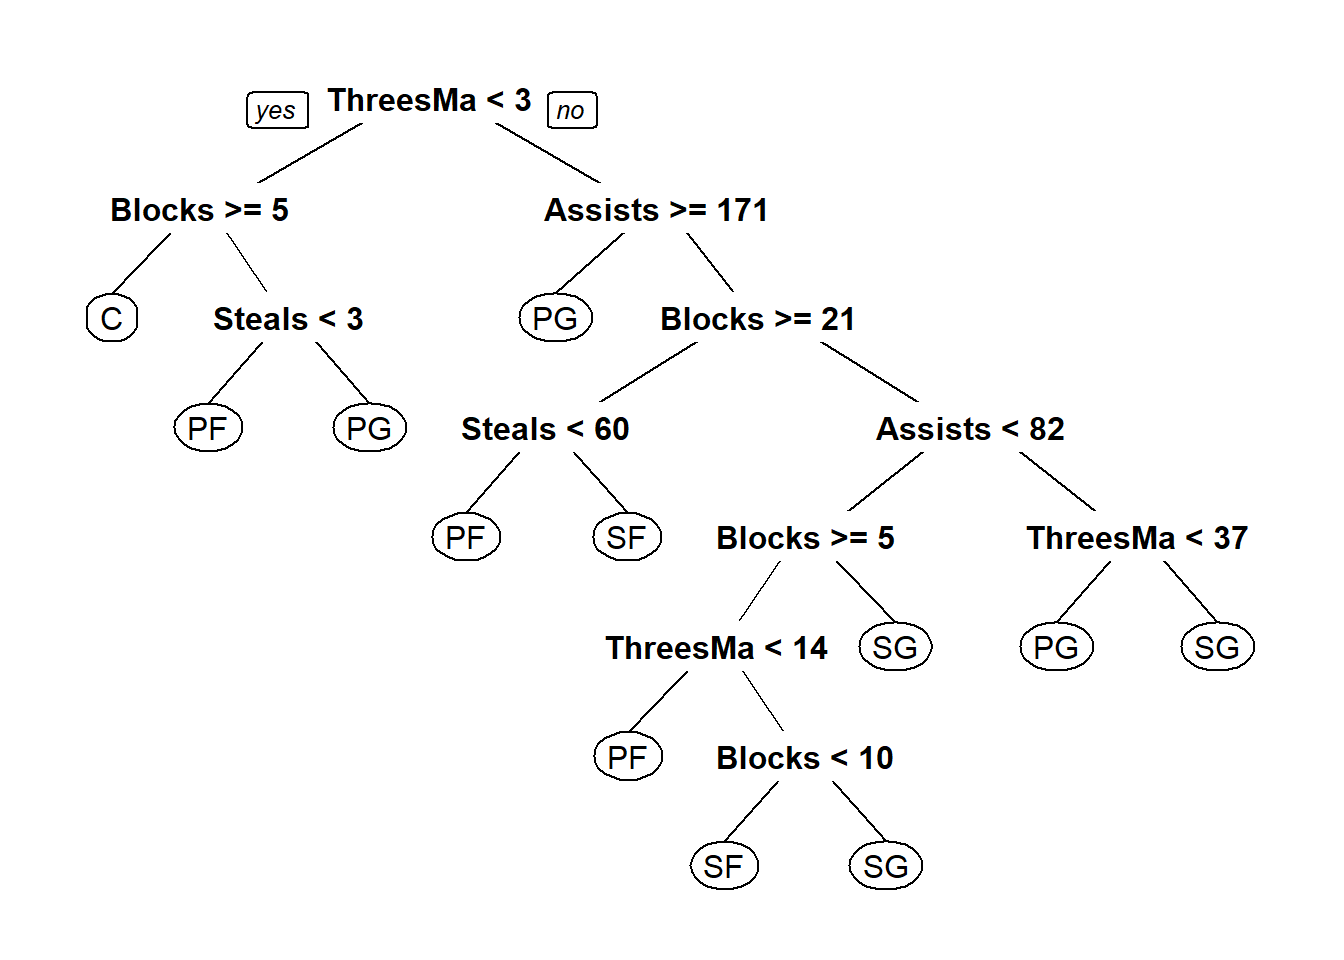
\includegraphics{DataAnalyticsWithR_files/figure-latex/unnamed-chunk-7-1.pdf}

Hierarchical Clustering -hclust()
用\texttt{hclust}函數畫圖,必要參數是個觀察職的距離(可用\texttt{dist()}函數計算)

\begin{Shaded}
\begin{Highlighting}[]
\KeywordTok{par}\NormalTok{(}\DataTypeTok{mar=}\KeywordTok{rep}\NormalTok{(}\DecValTok{2}\NormalTok{,}\DecValTok{4}\NormalTok{),}\DataTypeTok{mfrow=}\KeywordTok{c}\NormalTok{(}\DecValTok{1}\NormalTok{,}\DecValTok{1}\NormalTok{))}
\NormalTok{hc<-}\KeywordTok{hclust}\NormalTok{(}\KeywordTok{dist}\NormalTok{(mtcars.mxs),}\DataTypeTok{method=}\StringTok{"average"}\NormalTok{) }\CommentTok{#聚合方法為計算平均距離}
\KeywordTok{plot}\NormalTok{(hc)}
\end{Highlighting}
\end{Shaded}

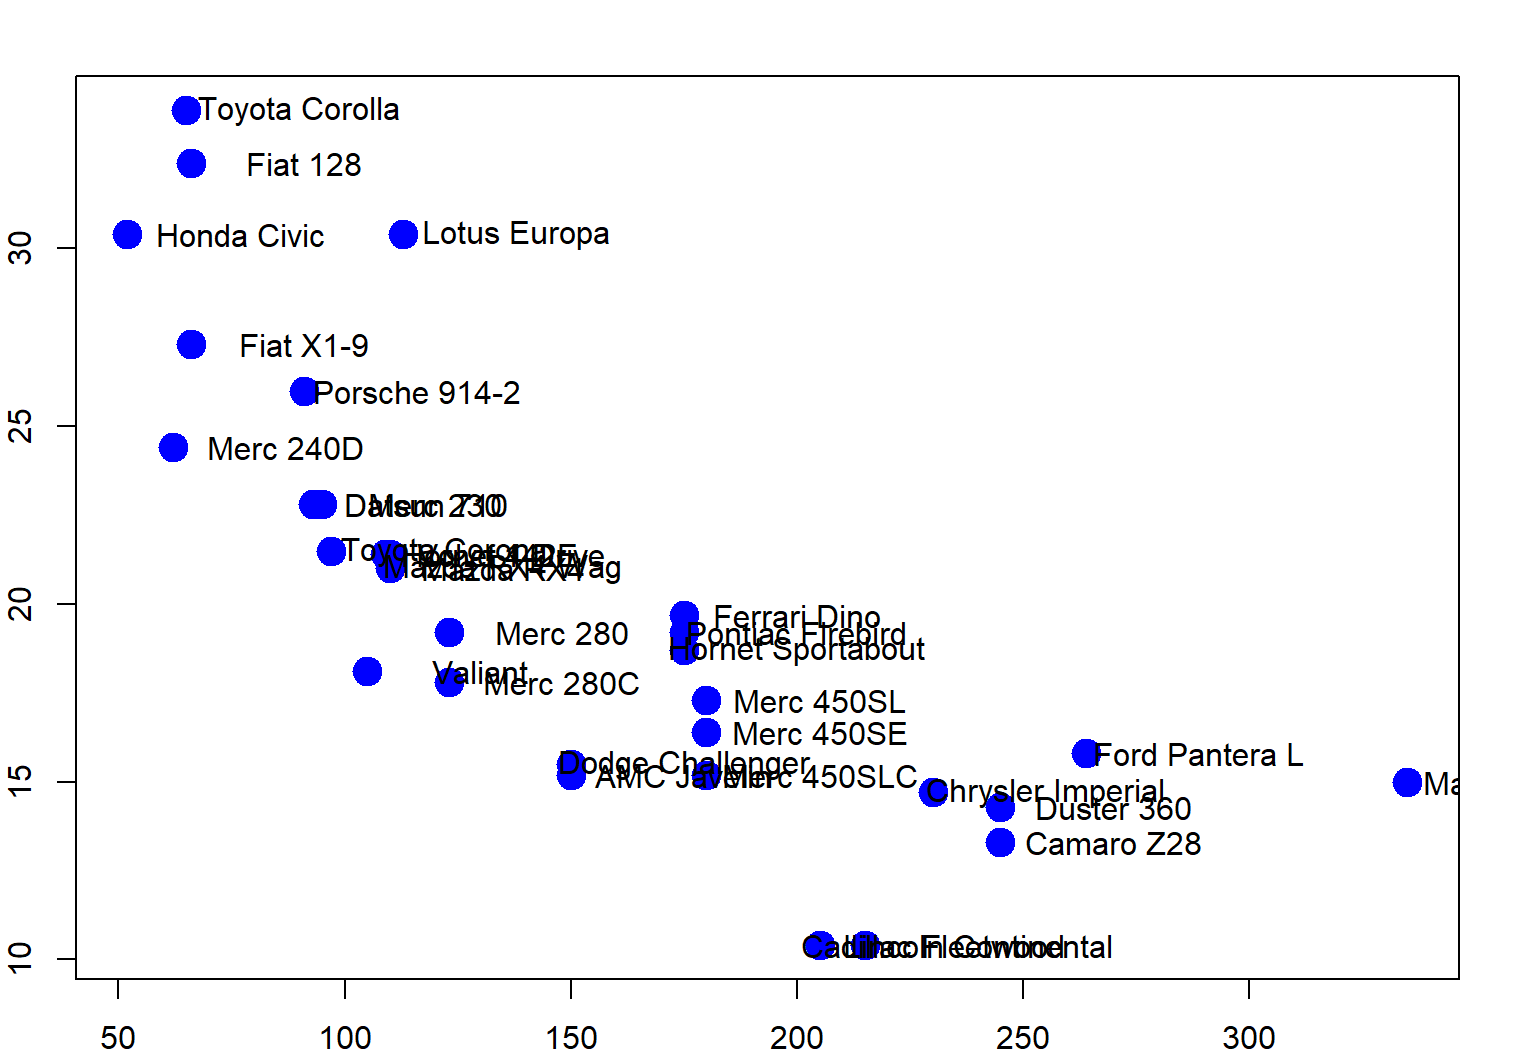
\includegraphics{DataAnalyticsWithR_files/figure-latex/unnamed-chunk-8-1.pdf}

Hierarchical Clustering -cutree()

\begin{Shaded}
\begin{Highlighting}[]
\NormalTok{clusterCut <-}\StringTok{ }\KeywordTok{cutree}\NormalTok{(hc, }\DataTypeTok{k=}\DecValTok{5}\NormalTok{) }\CommentTok{#分5群}
\KeywordTok{sort}\NormalTok{(clusterCut)}
\end{Highlighting}
\end{Shaded}

\begin{verbatim}
##           Mazda RX4       Mazda RX4 Wag          Datsun 710 
##                   1                   1                   1 
##           Merc 240D            Merc 230            Merc 280 
##                   1                   1                   1 
##           Merc 280C            Fiat 128         Honda Civic 
##                   1                   1                   1 
##      Toyota Corolla       Toyota Corona           Fiat X1-9 
##                   1                   1                   1 
##       Porsche 914-2        Lotus Europa        Ferrari Dino 
##                   1                   1                   1 
##          Volvo 142E      Hornet 4 Drive             Valiant 
##                   1                   2                   2 
##          Merc 450SE          Merc 450SL         Merc 450SLC 
##                   2                   2                   2 
##    Dodge Challenger         AMC Javelin   Hornet Sportabout 
##                   2                   2                   3 
##          Duster 360          Camaro Z28    Pontiac Firebird 
##                   3                   3                   3 
##      Ford Pantera L  Cadillac Fleetwood Lincoln Continental 
##                   3                   4                   4 
##   Chrysler Imperial       Maserati Bora 
##                   4                   5
\end{verbatim}

HC- clusters \& variables

\begin{Shaded}
\begin{Highlighting}[]
\KeywordTok{ggplot}\NormalTok{()+}\KeywordTok{geom_point}\NormalTok{(}\DataTypeTok{data=}\NormalTok{mtcars,}
                    \KeywordTok{aes}\NormalTok{(}\DataTypeTok{x=}\NormalTok{hp,}\DataTypeTok{y=}\NormalTok{mpg,}\DataTypeTok{color=}\KeywordTok{as.factor}\NormalTok{(clusterCut)))}
\end{Highlighting}
\end{Shaded}

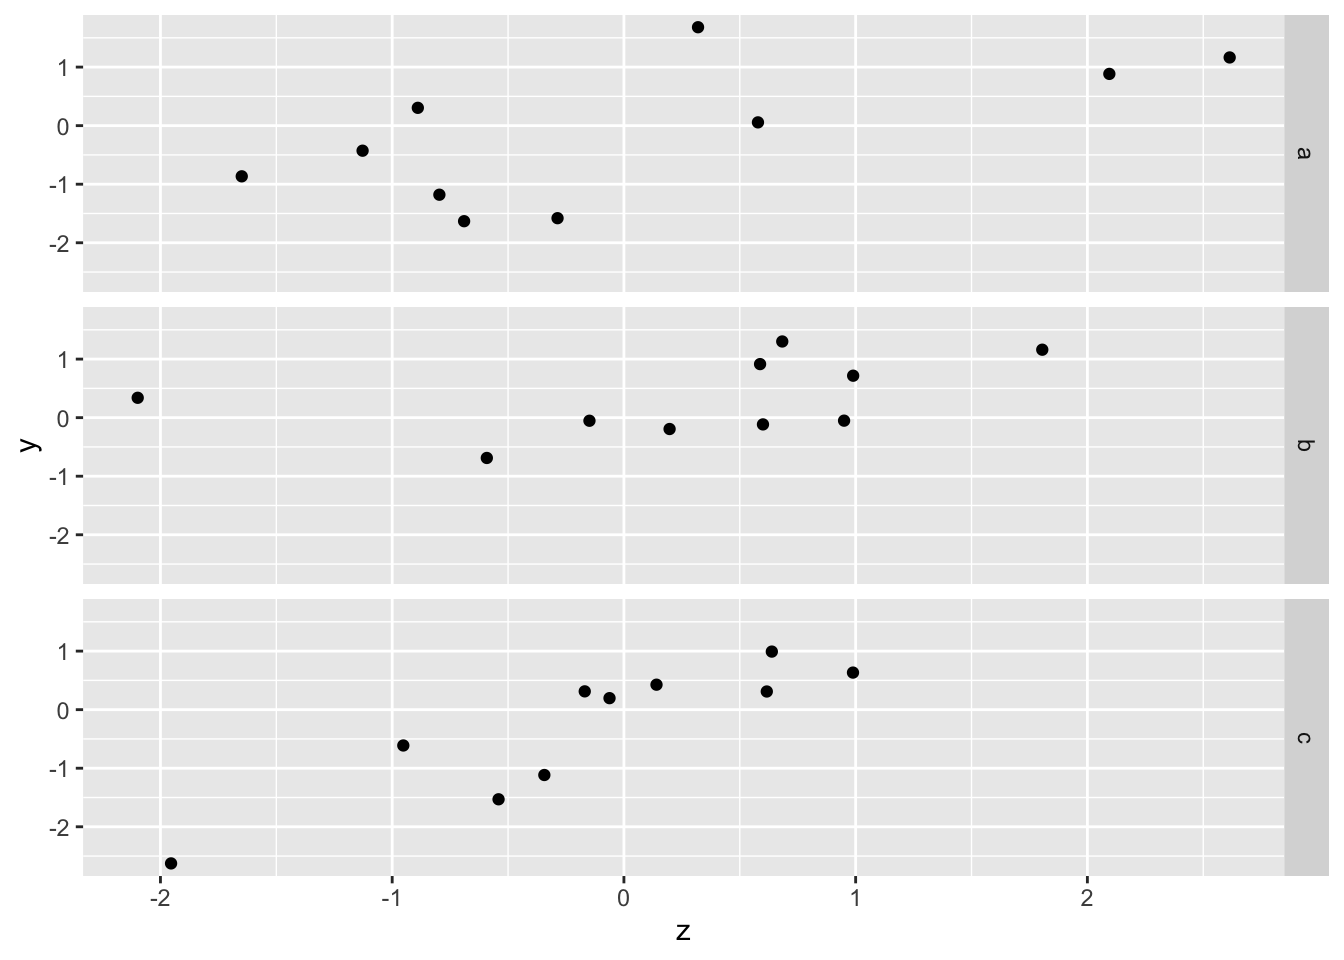
\includegraphics{DataAnalyticsWithR_files/figure-latex/unnamed-chunk-10-1.pdf}

Hierarchical Clustering -cutree(),2

\begin{Shaded}
\begin{Highlighting}[]
\NormalTok{clusterCut <-}\StringTok{ }\KeywordTok{cutree}\NormalTok{(hc,}\DataTypeTok{h =}\DecValTok{4}\NormalTok{) }\CommentTok{#切在高度=4的地方(距離=4)}
\KeywordTok{sort}\NormalTok{(clusterCut)}
\end{Highlighting}
\end{Shaded}

\begin{verbatim}
##           Mazda RX4       Mazda RX4 Wag          Datsun 710 
##                   1                   1                   2 
##      Hornet 4 Drive   Hornet Sportabout             Valiant 
##                   3                   4                   5 
##          Duster 360           Merc 240D            Merc 230 
##                   6                   7                   8 
##            Merc 280           Merc 280C          Merc 450SE 
##                   9                   9                  10 
##          Merc 450SL         Merc 450SLC  Cadillac Fleetwood 
##                  10                  10                  11 
## Lincoln Continental   Chrysler Imperial            Fiat 128 
##                  12                  13                  14 
##         Honda Civic      Toyota Corolla       Toyota Corona 
##                  15                  16                  17 
##    Dodge Challenger         AMC Javelin          Camaro Z28 
##                  18                  19                  20 
##    Pontiac Firebird           Fiat X1-9       Porsche 914-2 
##                  21                  22                  23 
##        Lotus Europa      Ford Pantera L        Ferrari Dino 
##                  24                  25                  26 
##       Maserati Bora          Volvo 142E 
##                  27                  28
\end{verbatim}

Cluster the data -heatmap(),2

\begin{Shaded}
\begin{Highlighting}[]
\KeywordTok{par}\NormalTok{(}\DataTypeTok{mar=}\KeywordTok{rep}\NormalTok{(}\FloatTok{0.2}\NormalTok{,}\DecValTok{4}\NormalTok{),}\DataTypeTok{mfrow=}\KeywordTok{c}\NormalTok{(}\DecValTok{1}\NormalTok{,}\DecValTok{1}\NormalTok{))}
\KeywordTok{heatmap}\NormalTok{(mtcars.mxs)}
\end{Highlighting}
\end{Shaded}

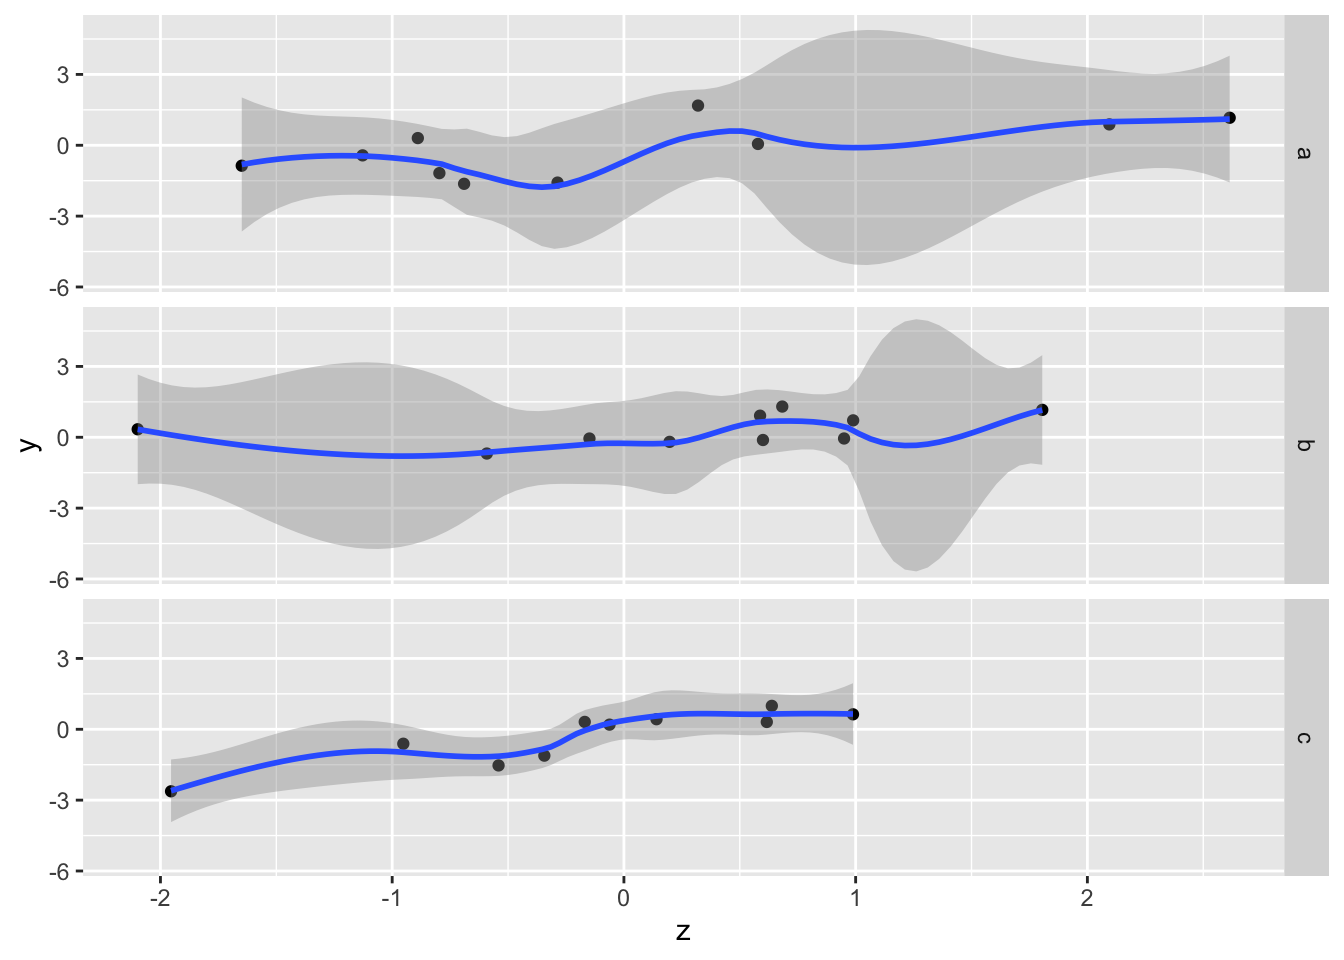
\includegraphics{DataAnalyticsWithR_files/figure-latex/unnamed-chunk-12-1.pdf}

Hierarchical clustering - hclust

\begin{Shaded}
\begin{Highlighting}[]
\NormalTok{distxy <-}\StringTok{ }\KeywordTok{dist}\NormalTok{(mtcars.mxs)}
\NormalTok{hClustering <-}\StringTok{ }\KeywordTok{hclust}\NormalTok{(distxy)}
\KeywordTok{plot}\NormalTok{(hClustering)}
\end{Highlighting}
\end{Shaded}

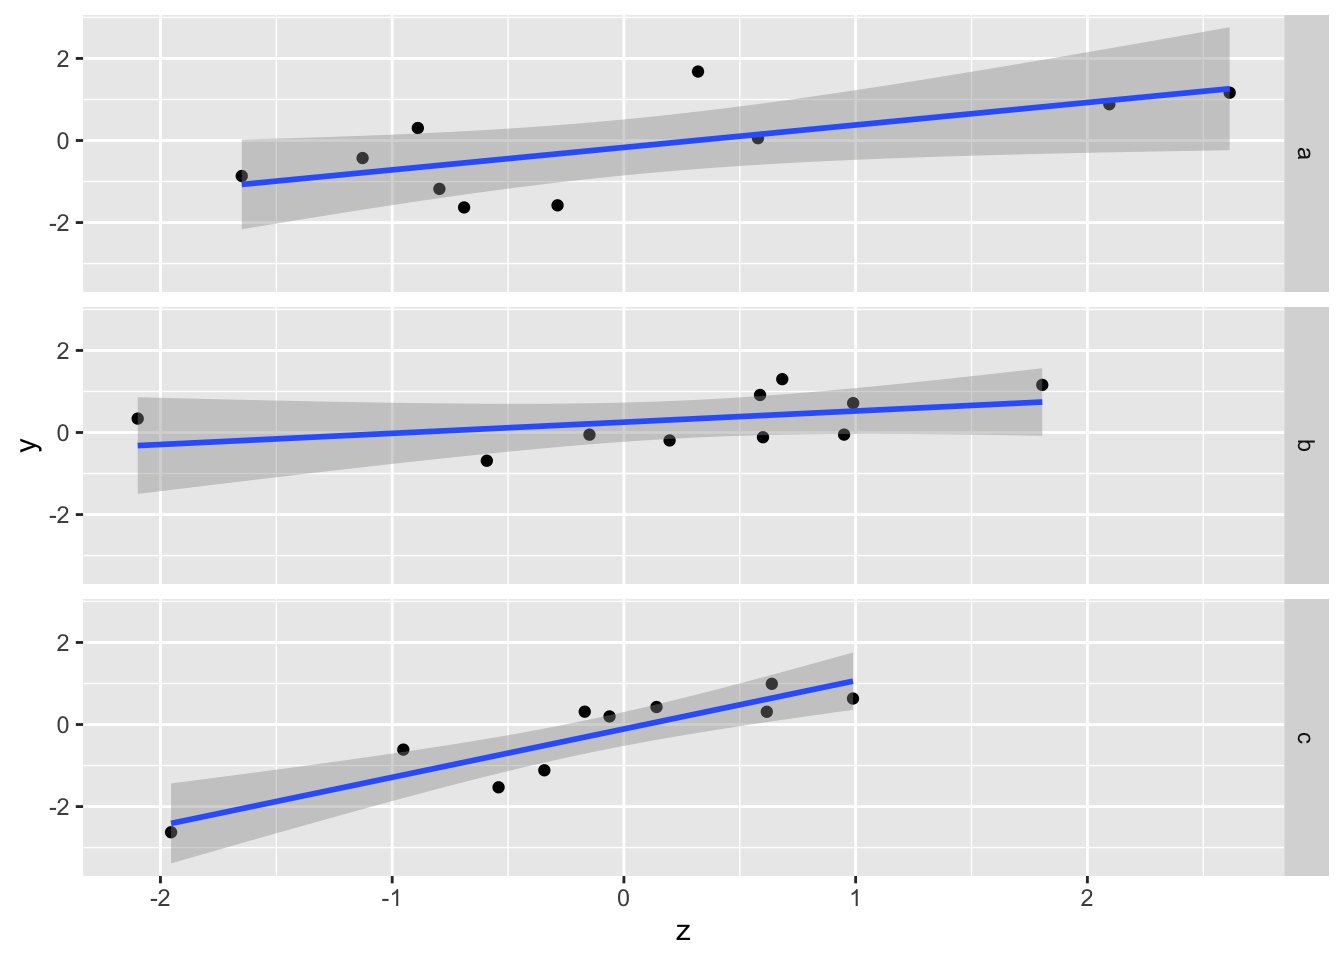
\includegraphics{DataAnalyticsWithR_files/figure-latex/unnamed-chunk-13-1.pdf}

Hierarchical clustering: summary - 可快速瀏覽觀察值與各欄位的關係

\begin{itemize}
\tightlist
\item
  分群結果可能被以下參數影響:

  \begin{itemize}
  \tightlist
  \item
    計算距離的方法
  \item
    分群依據
  \item
    更改數值的大小
  \end{itemize}
\item
  可能會遇到的問題:

  \begin{itemize}
  \tightlist
  \item
    有時會不太清楚要如何切割分群結果
  \end{itemize}
\end{itemize}

\subsubsection{K-means clustering}\label{k-means-clustering}

\begin{itemize}
\tightlist
\item
  執行步驟

  \begin{itemize}
  \tightlist
  \item
    指定要分幾群
  \item
    計算每一群的中心點
  \item
    將各個物件/觀察值指定給最近的中心點
  \item
    依照新的分群計算新的中心點
  \end{itemize}
\item
  輸入

  \begin{itemize}
  \tightlist
  \item
    計算距離的資料(數值)
  \item
    要分成幾群 \# of clusters
  \item
    預設個群的中間點位置
  \end{itemize}
\item
  產出

  \begin{itemize}
  \tightlist
  \item
    計算出每'群`的中心點
  \item
    指定每個觀察值所在的'群`
  \end{itemize}
\end{itemize}

\begin{Shaded}
\begin{Highlighting}[]
\NormalTok{x<-}\KeywordTok{scale}\NormalTok{(mtcars$hp[-}\DecValTok{1}\NormalTok{]);y<-}\KeywordTok{scale}\NormalTok{(mtcars$mpg[-}\DecValTok{1}\NormalTok{])}
\KeywordTok{plot}\NormalTok{(x,y,}\DataTypeTok{col=}\StringTok{"blue"}\NormalTok{,}\DataTypeTok{pch=}\DecValTok{19}\NormalTok{,}\DataTypeTok{cex=}\DecValTok{2}\NormalTok{)}
\KeywordTok{text}\NormalTok{(x}\FloatTok{+0.05}\NormalTok{,y}\FloatTok{+0.05}\NormalTok{,}\DataTypeTok{labels=}\NormalTok{labelCar)}
\end{Highlighting}
\end{Shaded}

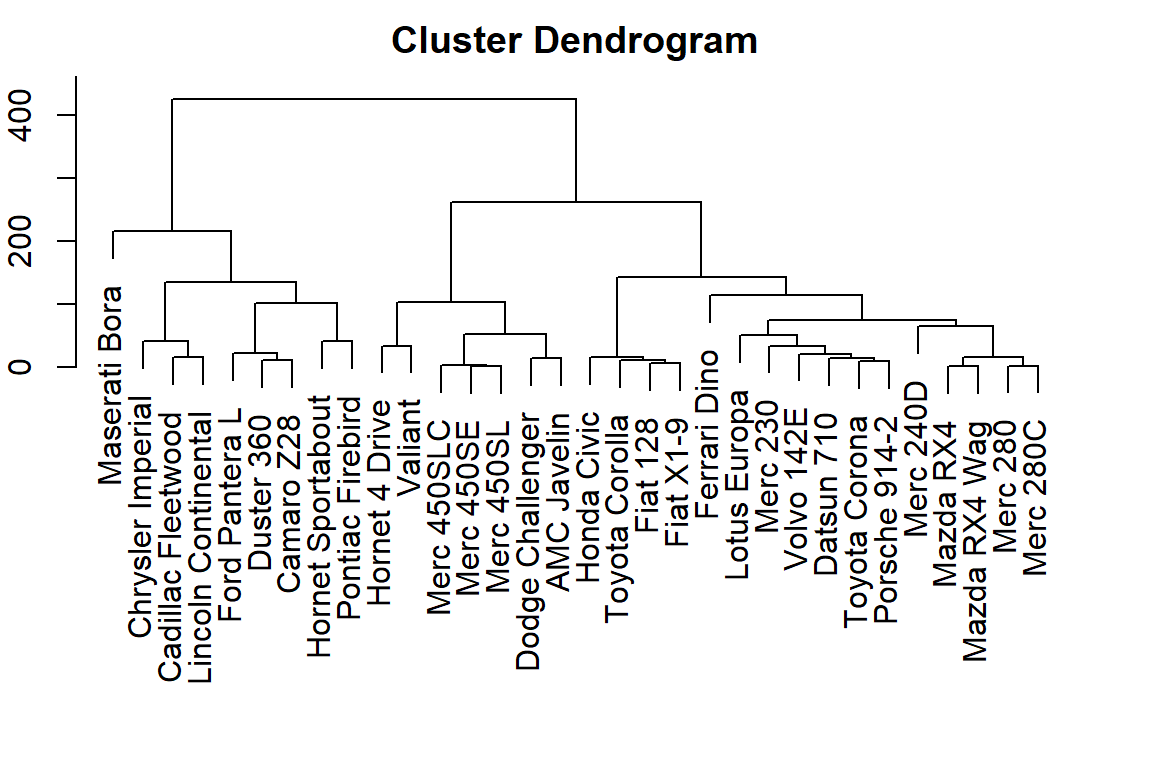
\includegraphics{DataAnalyticsWithR_files/figure-latex/unnamed-chunk-14-1.pdf}

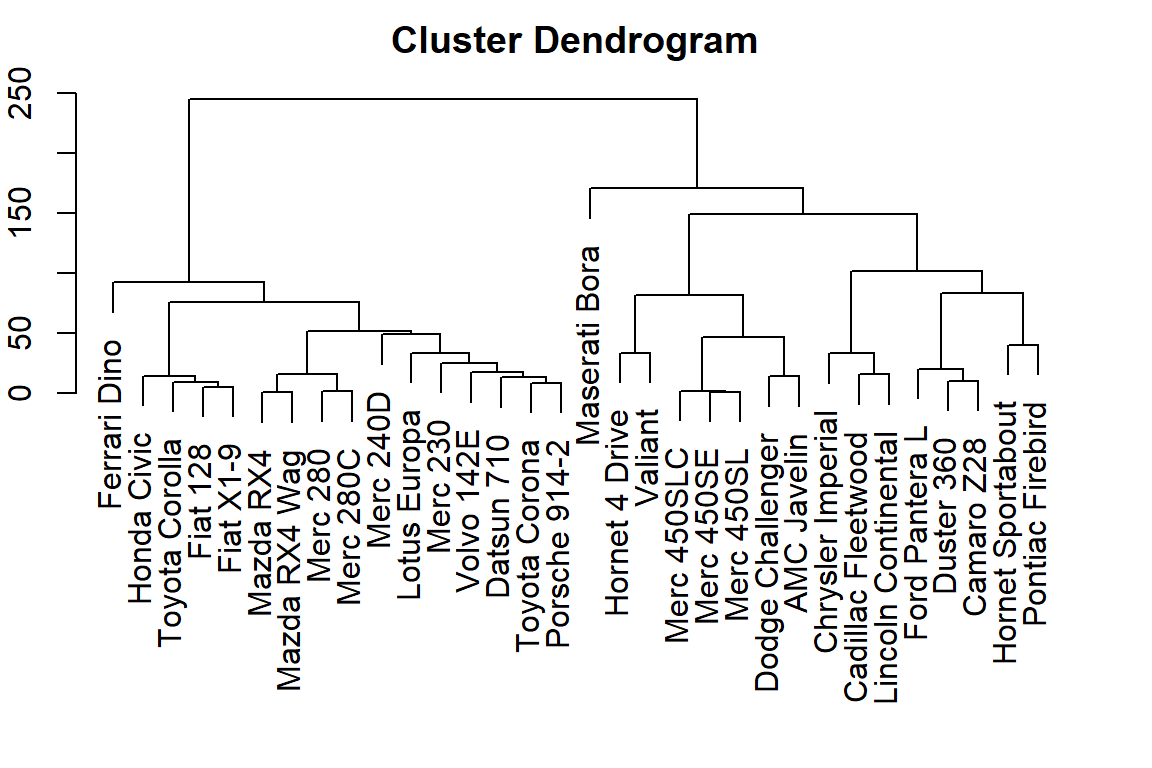
\includegraphics{DataAnalyticsWithR_files/figure-latex/unnamed-chunk-15-1.pdf}

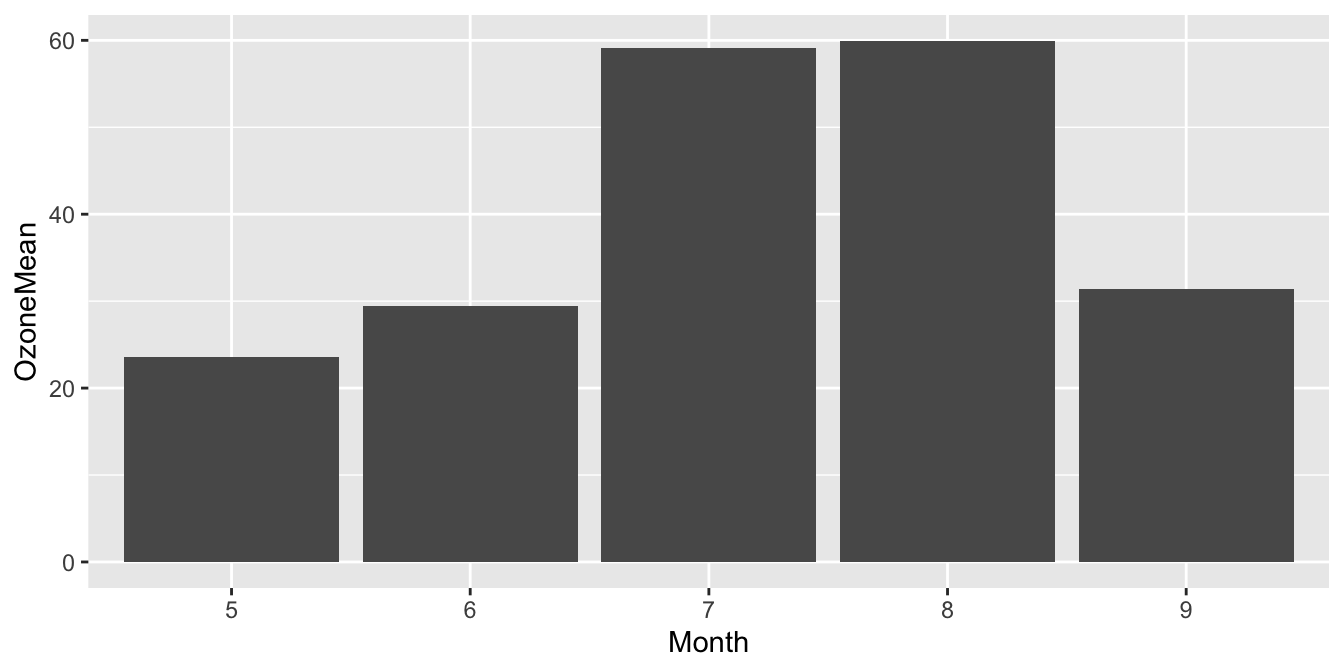
\includegraphics{DataAnalyticsWithR_files/figure-latex/unnamed-chunk-16-1.pdf}

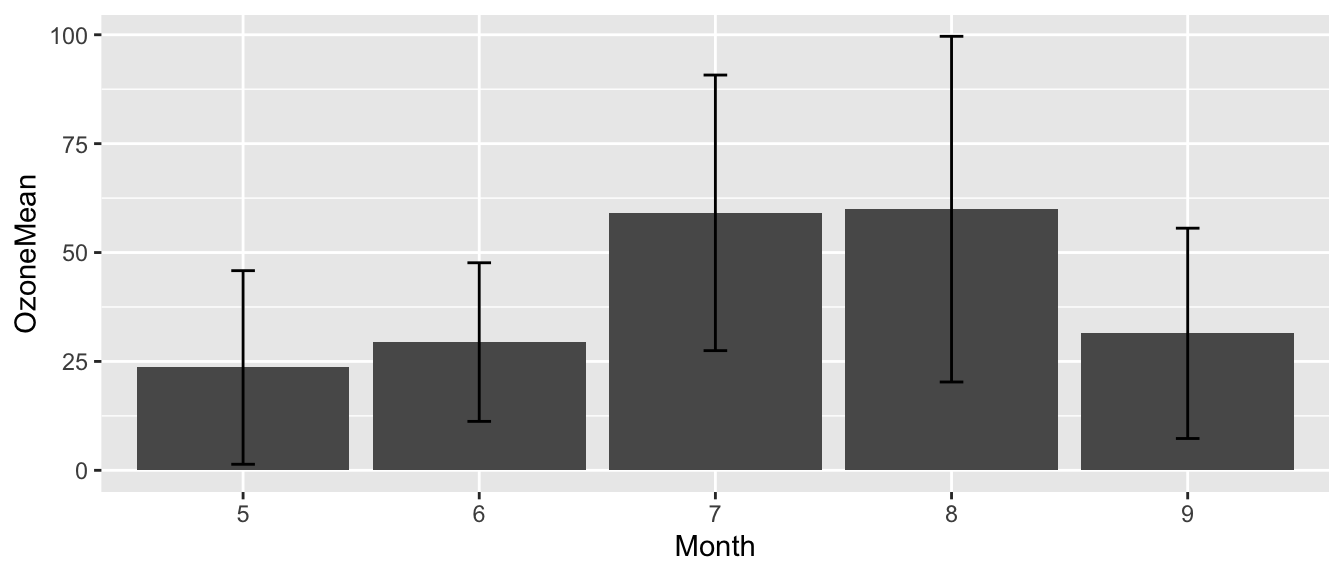
\includegraphics{DataAnalyticsWithR_files/figure-latex/unnamed-chunk-17-1.pdf}

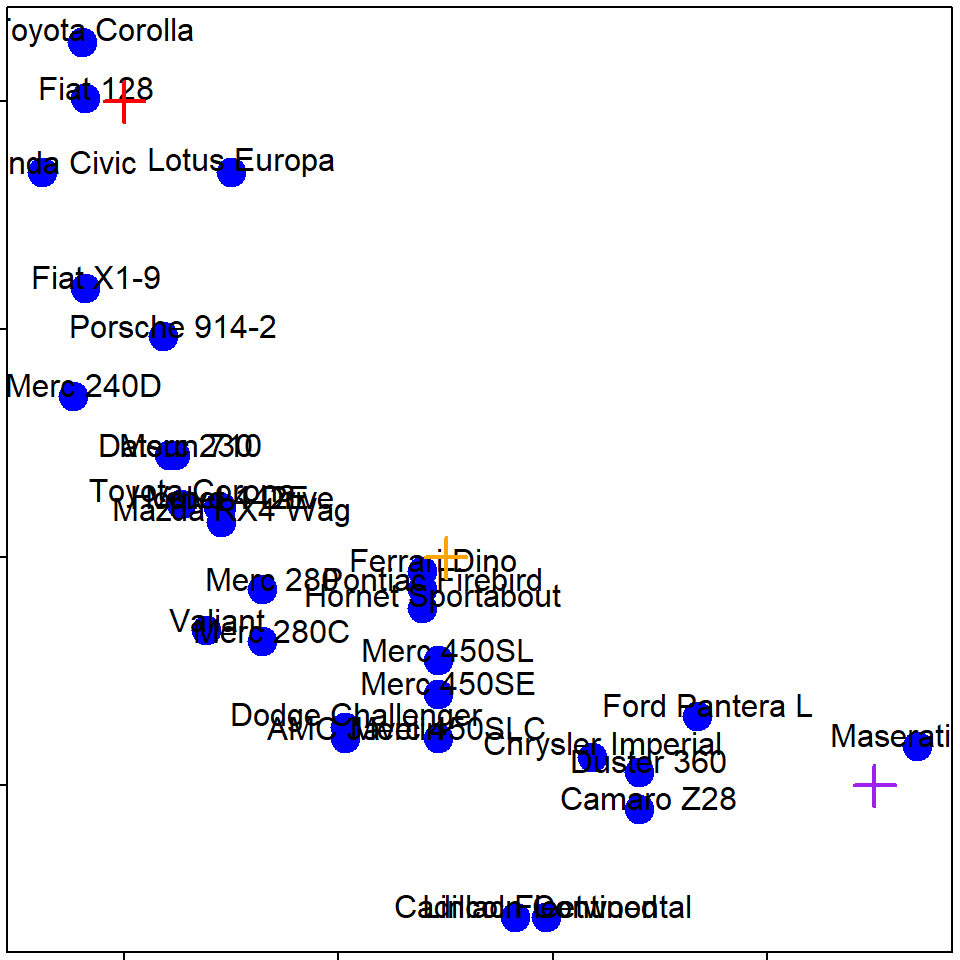
\includegraphics{DataAnalyticsWithR_files/figure-latex/unnamed-chunk-18-1.pdf}

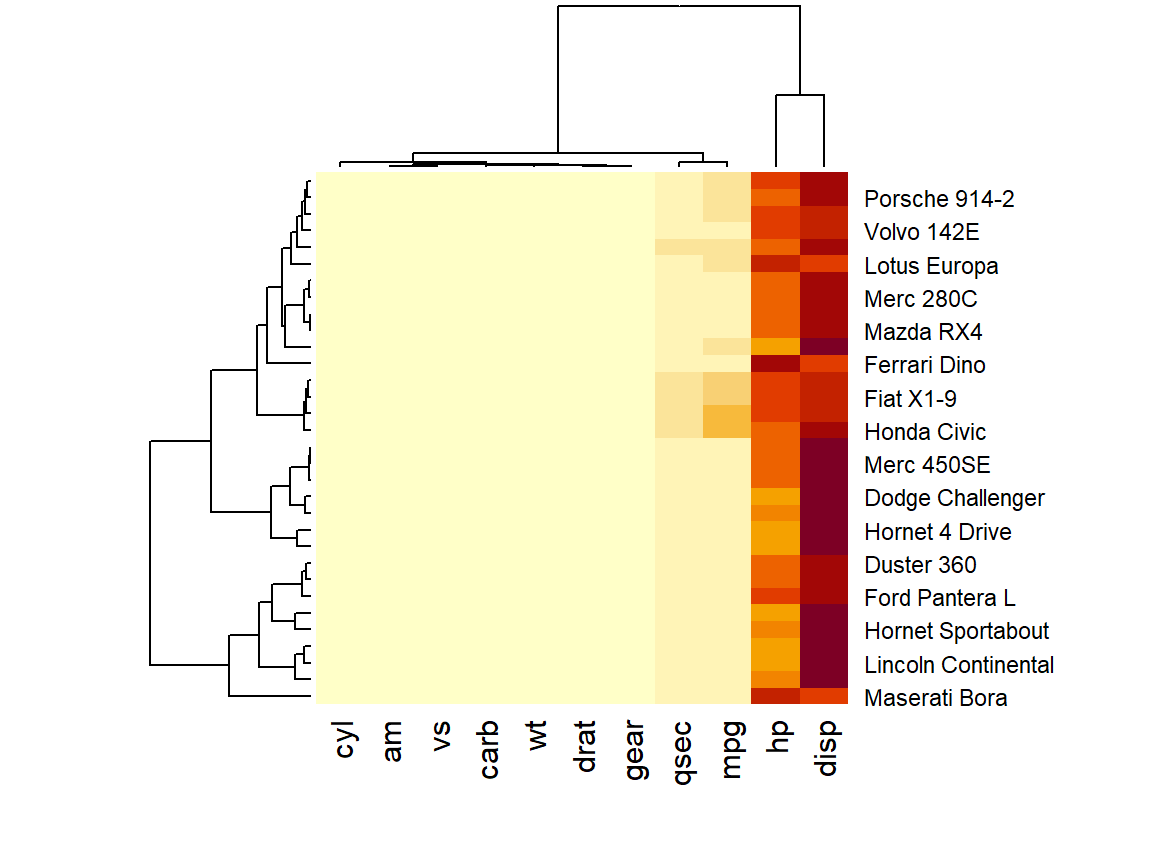
\includegraphics{DataAnalyticsWithR_files/figure-latex/unnamed-chunk-19-1.pdf}

\texttt{kmeans()}

\begin{itemize}
\tightlist
\item
  Important parameters: \texttt{x}, \texttt{centers}, \texttt{iter.max},
  \texttt{nstart}
\end{itemize}

\begin{Shaded}
\begin{Highlighting}[]
\NormalTok{dataFrame <-}\StringTok{ }\KeywordTok{data.frame}\NormalTok{(x,y)}
\NormalTok{kmeansObj <-}\StringTok{ }\KeywordTok{kmeans}\NormalTok{(dataFrame,}\DataTypeTok{centers=}\DecValTok{3}\NormalTok{)}
\KeywordTok{names}\NormalTok{(kmeansObj)}
\end{Highlighting}
\end{Shaded}

\begin{verbatim}
## [1] "cluster"      "centers"      "totss"        "withinss"    
## [5] "tot.withinss" "betweenss"    "size"         "iter"        
## [9] "ifault"
\end{verbatim}

\begin{Shaded}
\begin{Highlighting}[]
\NormalTok{kmeansObj$cluster}
\end{Highlighting}
\end{Shaded}

\begin{verbatim}
##  [1] 2 2 2 2 2 3 1 2 2 2 2 2 2 3 3 3 1 1 1 2 2 2 3 2 1 1 1 3 2 3 2
\end{verbatim}

\begin{Shaded}
\begin{Highlighting}[]
\KeywordTok{par}\NormalTok{(}\DataTypeTok{mar=}\KeywordTok{rep}\NormalTok{(}\FloatTok{0.2}\NormalTok{,}\DecValTok{4}\NormalTok{))}
\KeywordTok{plot}\NormalTok{(x,y,}\DataTypeTok{col=}\NormalTok{kmeansObj$cluster,}\DataTypeTok{pch=}\DecValTok{19}\NormalTok{,}\DataTypeTok{cex=}\DecValTok{2}\NormalTok{)}
\KeywordTok{points}\NormalTok{(kmeansObj$centers,}\DataTypeTok{col=}\DecValTok{1}\NormalTok{:}\DecValTok{3}\NormalTok{,}\DataTypeTok{pch=}\DecValTok{3}\NormalTok{,}\DataTypeTok{cex=}\DecValTok{3}\NormalTok{,}\DataTypeTok{lwd=}\DecValTok{3}\NormalTok{)}
\end{Highlighting}
\end{Shaded}

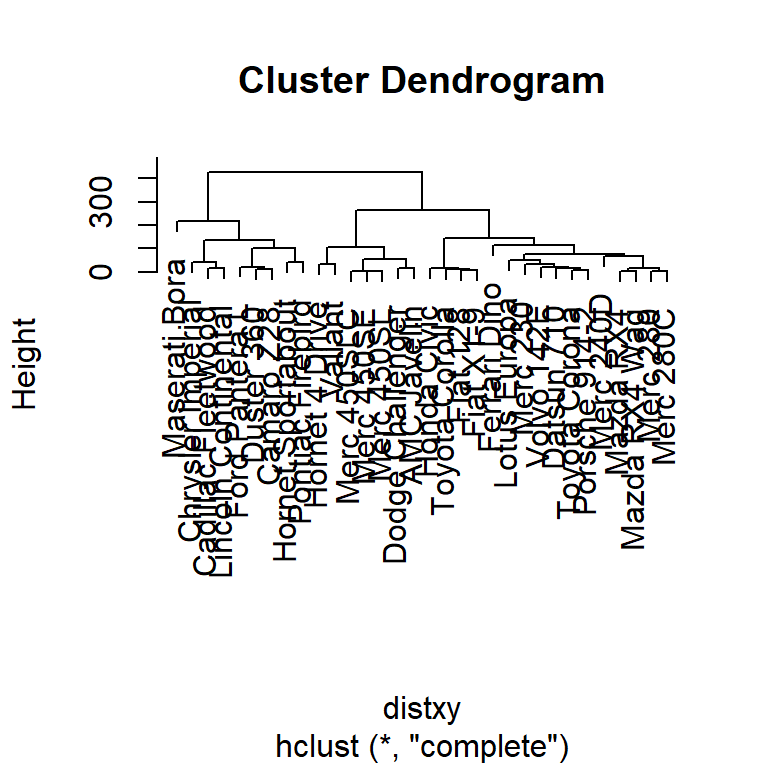
\includegraphics{DataAnalyticsWithR_files/figure-latex/unnamed-chunk-20-1.pdf}

Heatmaps

\begin{Shaded}
\begin{Highlighting}[]
\KeywordTok{set.seed}\NormalTok{(}\DecValTok{1234}\NormalTok{)}
\NormalTok{dataMatrix <-}\StringTok{ }\KeywordTok{as.matrix}\NormalTok{(dataFrame)[}\KeywordTok{sample}\NormalTok{(}\DecValTok{1}\NormalTok{:}\DecValTok{12}\NormalTok{),]}
\NormalTok{kmeansObj <-}\StringTok{ }\KeywordTok{kmeans}\NormalTok{(dataMatrix,}\DataTypeTok{centers=}\DecValTok{3}\NormalTok{)}
\KeywordTok{par}\NormalTok{(}\DataTypeTok{mfrow=}\KeywordTok{c}\NormalTok{(}\DecValTok{1}\NormalTok{,}\DecValTok{2}\NormalTok{), }\DataTypeTok{mar =} \KeywordTok{c}\NormalTok{(}\DecValTok{2}\NormalTok{, }\DecValTok{4}\NormalTok{, }\FloatTok{0.1}\NormalTok{, }\FloatTok{0.1}\NormalTok{))}
\KeywordTok{image}\NormalTok{(}\KeywordTok{t}\NormalTok{(dataMatrix)[,}\KeywordTok{nrow}\NormalTok{(dataMatrix):}\DecValTok{1}\NormalTok{],}\DataTypeTok{yaxt=}\StringTok{"n"}\NormalTok{)}
\KeywordTok{image}\NormalTok{(}\KeywordTok{t}\NormalTok{(dataMatrix)[,}\KeywordTok{order}\NormalTok{(kmeansObj$cluster)],}\DataTypeTok{yaxt=}\StringTok{"n"}\NormalTok{)}
\end{Highlighting}
\end{Shaded}

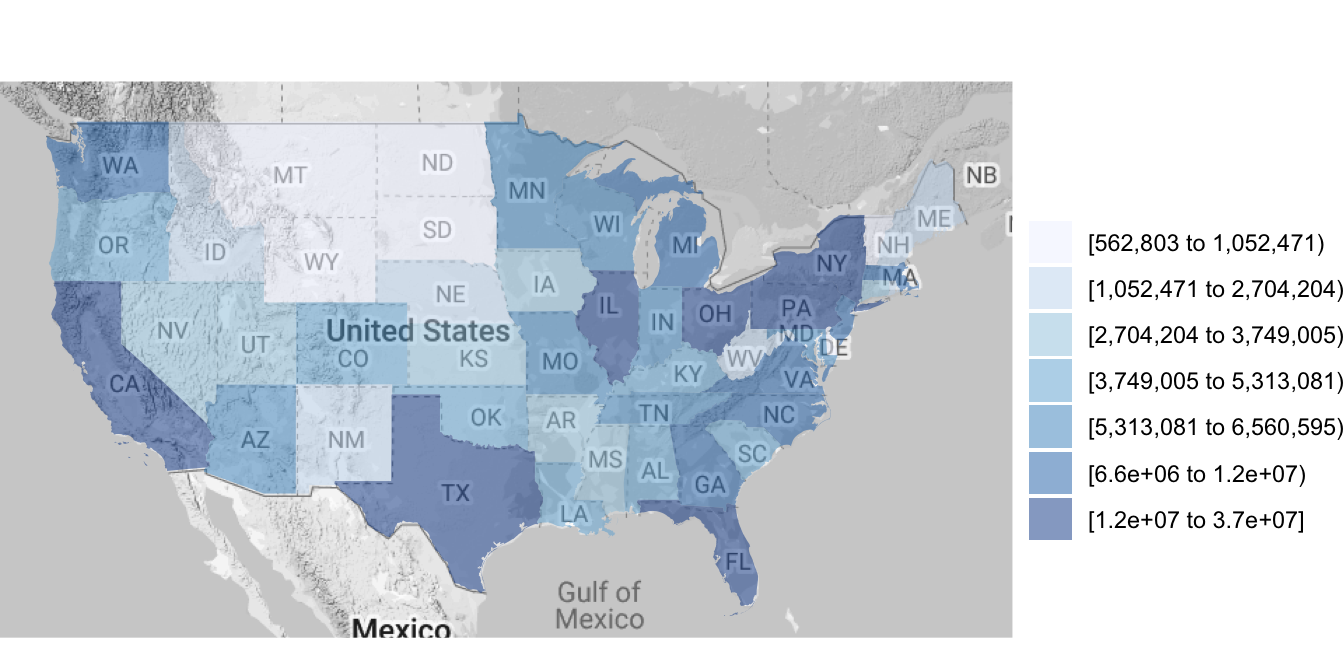
\includegraphics{DataAnalyticsWithR_files/figure-latex/unnamed-chunk-21-1.pdf}

K-means注意事項

\begin{itemize}
\tightlist
\item
  需要決定\# of clusters

  \begin{itemize}
  \tightlist
  \item
    用眼睛/人工/特殊要求選
  \item
    用 cross validation/information theory選
  \item
    \href{http://en.wikipedia.org/wiki/Determining_the_number_of_clusters_in_a_data_set}{Determining
    the number of clusters}
  \end{itemize}
\item
  K-means 沒有一定的結果

  \begin{itemize}
  \tightlist
  \item
    不同的 \# of clusters
  \item
    不同的 \# of iterations
  \end{itemize}
\end{itemize}

\texttt{kmeans()}, k=2

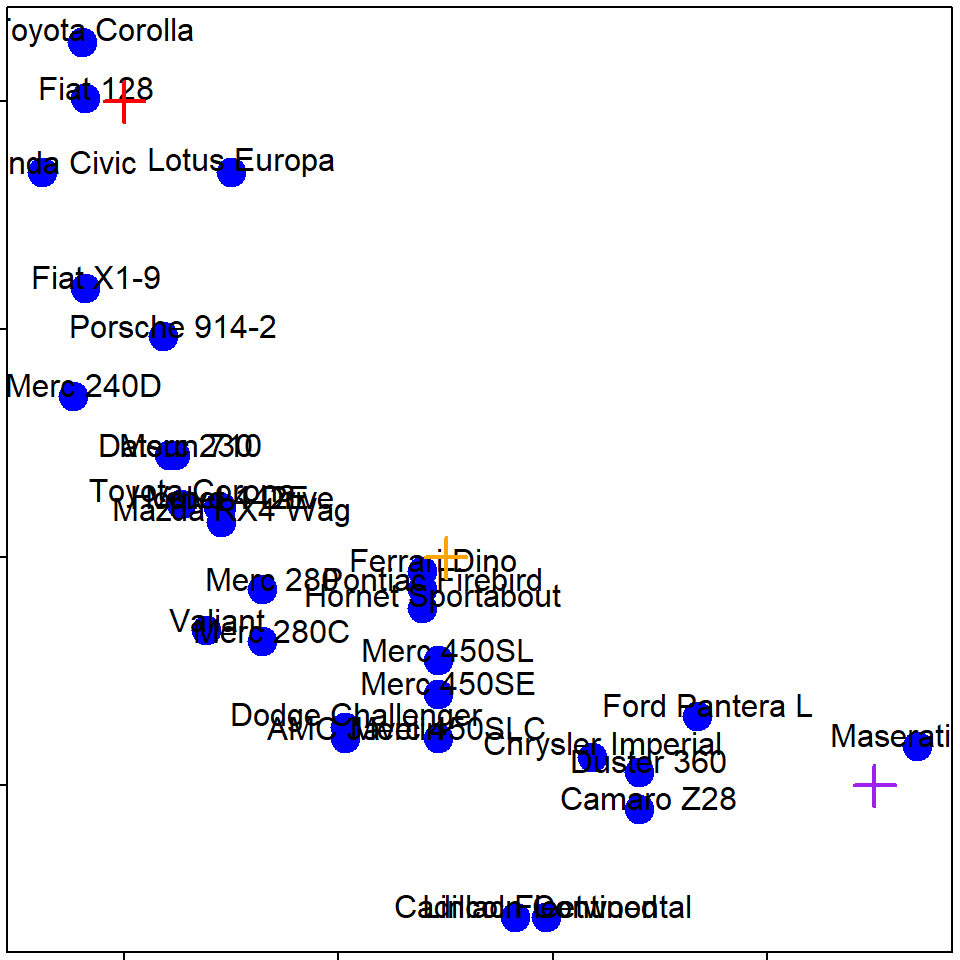
\includegraphics{DataAnalyticsWithR_files/figure-latex/unnamed-chunk-22-1.pdf}

\texttt{kmeans()}, k=3

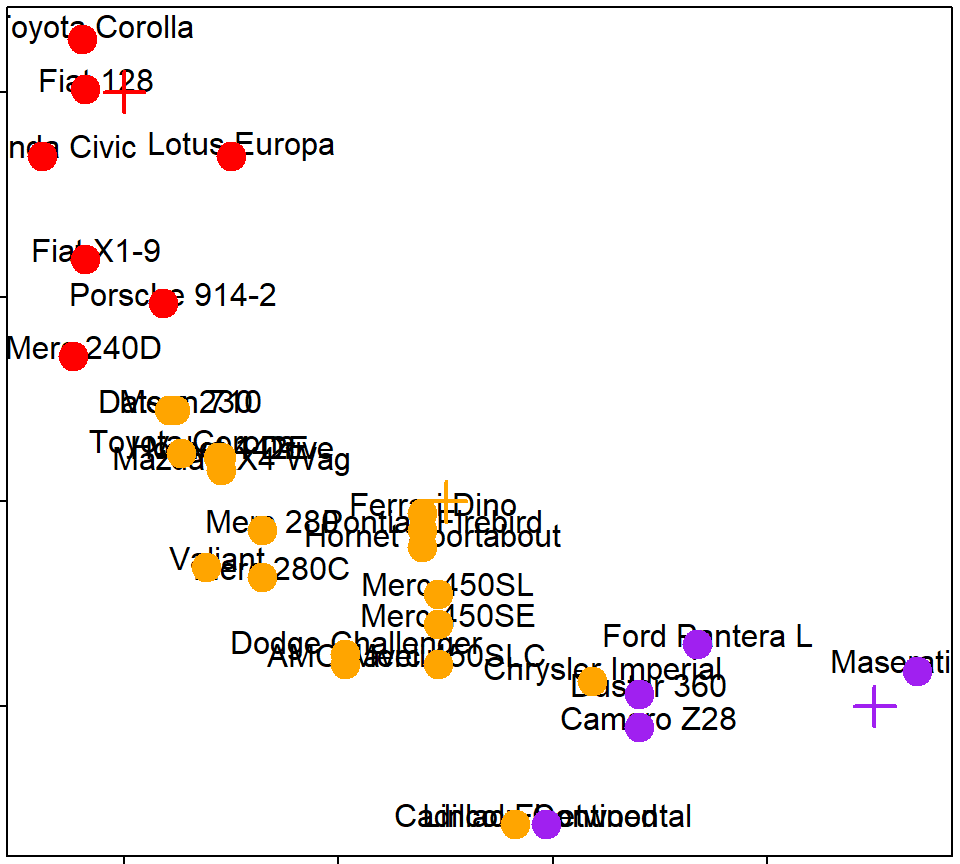
\includegraphics{DataAnalyticsWithR_files/figure-latex/unnamed-chunk-23-1.pdf}

\texttt{kmeans()}, k=4

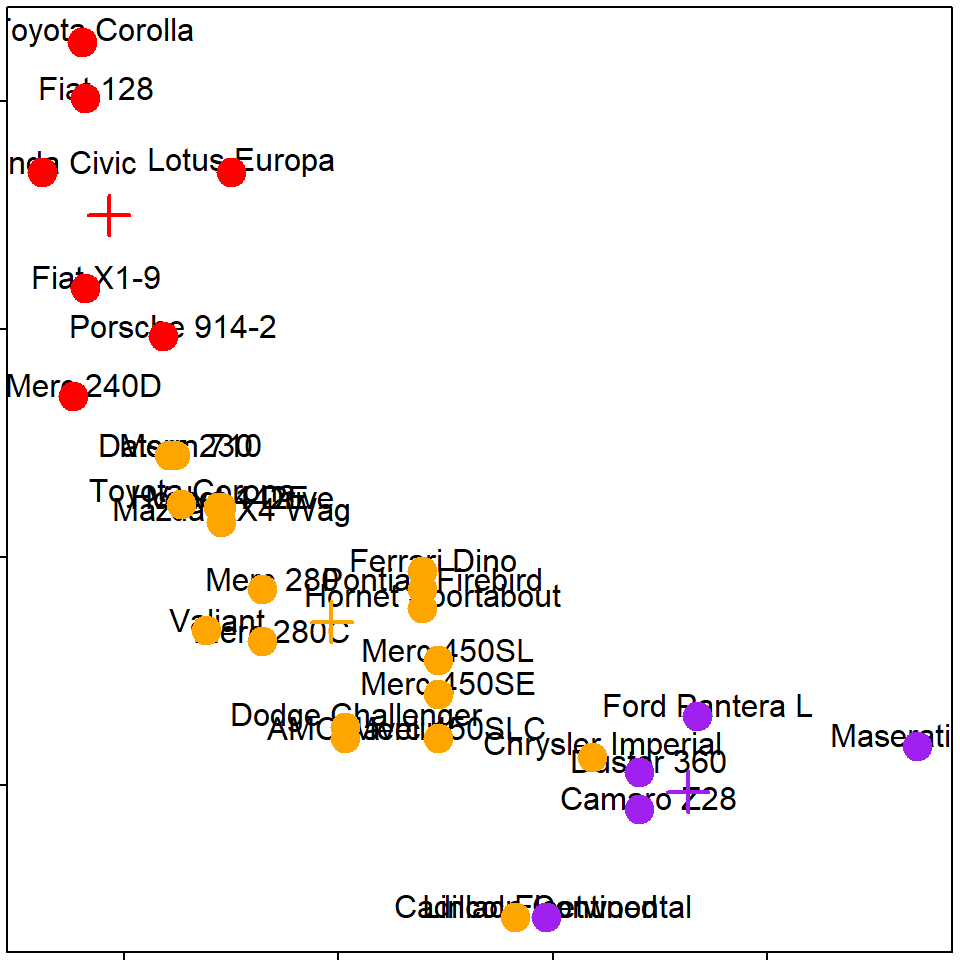
\includegraphics{DataAnalyticsWithR_files/figure-latex/unnamed-chunk-24-1.pdf}

Use sum of squared error (SSE) scree plot to optimize the number of
clusters

SSE: The sum of the squared distance between each member of a cluster
and its cluster centroid.

\href{http://stackoverflow.com/questions/15376075/cluster-analysis-in-r-determine-the-optimal-number-of-clusters}{參考資料}

SSE screen plot \texttt{withinss}

\begin{Shaded}
\begin{Highlighting}[]
\NormalTok{dataMatrix <-}\StringTok{ }\KeywordTok{as.matrix}\NormalTok{(dataFrame)[}\KeywordTok{sample}\NormalTok{(}\DecValTok{1}\NormalTok{:}\DecValTok{12}\NormalTok{),]}
\NormalTok{wss <-}\StringTok{ }\NormalTok{(}\KeywordTok{nrow}\NormalTok{(dataMatrix)-}\DecValTok{1}\NormalTok{)*}\KeywordTok{sum}\NormalTok{(}\KeywordTok{apply}\NormalTok{(dataMatrix,}\DecValTok{2}\NormalTok{,var))}
\NormalTok{for (i in }\DecValTok{2}\NormalTok{:(}\KeywordTok{nrow}\NormalTok{(dataMatrix)-}\DecValTok{1}\NormalTok{)) \{}
    \NormalTok{wss[i] <-}\StringTok{ }\KeywordTok{sum}\NormalTok{(}\KeywordTok{kmeans}\NormalTok{(dataMatrix,}\DataTypeTok{centers=}\NormalTok{i)$withinss)}
\NormalTok{\}}
\KeywordTok{par}\NormalTok{(}\DataTypeTok{mfrow=}\KeywordTok{c}\NormalTok{(}\DecValTok{1}\NormalTok{,}\DecValTok{1}\NormalTok{), }\DataTypeTok{mar =} \KeywordTok{c}\NormalTok{(}\DecValTok{4}\NormalTok{,}\DecValTok{4}\NormalTok{,}\DecValTok{1}\NormalTok{,}\DecValTok{1}\NormalTok{)) }\CommentTok{#下,左,上,右}
\KeywordTok{plot}\NormalTok{(}\DecValTok{1}\NormalTok{:(}\KeywordTok{nrow}\NormalTok{(dataMatrix)-}\DecValTok{1}\NormalTok{), wss, }\DataTypeTok{type=}\StringTok{"b"}\NormalTok{, }\DataTypeTok{xlab=}\StringTok{"Number of Clusters"}\NormalTok{,}
     \DataTypeTok{ylab=}\StringTok{"Within groups sum of squares"}\NormalTok{)}
\end{Highlighting}
\end{Shaded}

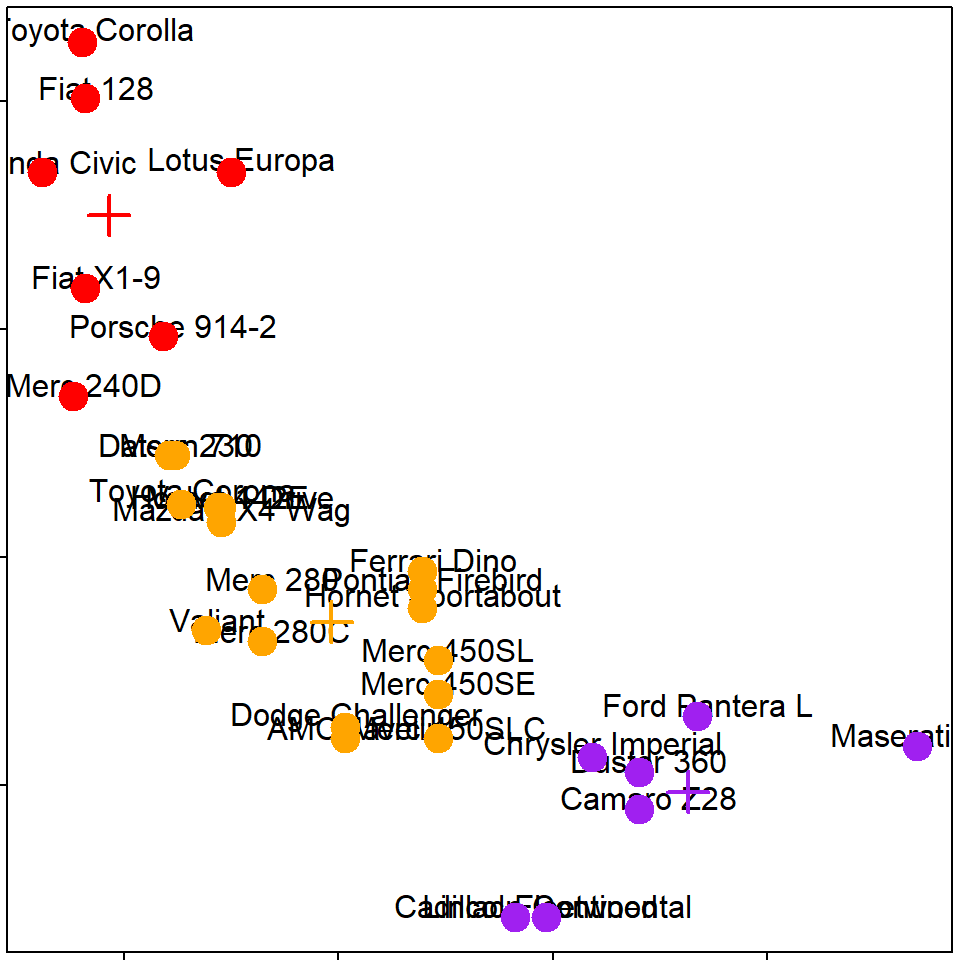
\includegraphics{DataAnalyticsWithR_files/figure-latex/unnamed-chunk-25-1.pdf}

\subsection{Association Rules 關聯式規則}\label{association-rules-}

什麼是關聯式規則? - 用於從大量數據中挖掘出有價值的數據項之間的相關關係
- 不考慮項目的次序,而僅考慮其組合 -
\texttt{購物籃分析\ (Market\ Basket\ Analysis)} -
Apriori演算法是挖掘\texttt{布林關聯規則} (Boolean association rules)
頻繁項集的算法

Apriori演算法

超市資料分析:讀取資料

\begin{Shaded}
\begin{Highlighting}[]
\CommentTok{# Load the libraries}
\NormalTok{if (!}\KeywordTok{require}\NormalTok{(}\StringTok{'arules'}\NormalTok{))\{}
    \KeywordTok{install.packages}\NormalTok{(}\StringTok{"arules"}\NormalTok{);}\KeywordTok{library}\NormalTok{(arules) }\CommentTok{#for Apriori演算法}
\NormalTok{\}}
\NormalTok{if (!}\KeywordTok{require}\NormalTok{(}\StringTok{'datasets'}\NormalTok{))\{}
    \KeywordTok{install.packages}\NormalTok{(}\StringTok{"datasets"}\NormalTok{);}\KeywordTok{library}\NormalTok{(datasets) }\CommentTok{#for Groceries data}
\NormalTok{\}}
\KeywordTok{data}\NormalTok{(Groceries) }\CommentTok{# Load the data set}
\NormalTok{Groceries@data@Dim }\CommentTok{#169 種商品,9835筆交易資料}
\end{Highlighting}
\end{Shaded}

\begin{verbatim}
## [1]  169 9835
\end{verbatim}

超市資料長這樣

超市資料分析:關聯式分析\texttt{apriori()}

\begin{Shaded}
\begin{Highlighting}[]
\CommentTok{# Get the rules}
\NormalTok{rules <-}\StringTok{ }\KeywordTok{apriori}\NormalTok{(Groceries, }\CommentTok{# data= Groceries}
                 \DataTypeTok{parameter =} \KeywordTok{list}\NormalTok{(}\DataTypeTok{supp =} \FloatTok{0.001}\NormalTok{, }\DataTypeTok{conf =} \FloatTok{0.8}\NormalTok{), }\CommentTok{#參數最低限度}
                 \DataTypeTok{control =} \KeywordTok{list}\NormalTok{(}\DataTypeTok{verbose=}\NormalTok{F)) }\CommentTok{#不要顯示output}
\KeywordTok{options}\NormalTok{(}\DataTypeTok{digits=}\DecValTok{2}\NormalTok{) }\CommentTok{# Only 2 digits}
\KeywordTok{inspect}\NormalTok{(rules[}\DecValTok{1}\NormalTok{:}\DecValTok{5}\NormalTok{]) }\CommentTok{# Show the top 5 rules}
\end{Highlighting}
\end{Shaded}

\begin{verbatim}
##     lhs                        rhs            support confidence lift
## [1] {liquor,red/blush wine} => {bottled beer} 0.0019  0.90       11.2
## [2] {curd,cereals}          => {whole milk}   0.0010  0.91        3.6
## [3] {yogurt,cereals}        => {whole milk}   0.0017  0.81        3.2
## [4] {butter,jam}            => {whole milk}   0.0010  0.83        3.3
## [5] {soups,bottled beer}    => {whole milk}   0.0011  0.92        3.6
\end{verbatim}

如何解讀模型 啤酒=\textgreater{}尿布

\begin{itemize}
\tightlist
\item
  \texttt{Support}:
  一次交易中,包括規則內的物品的機率。買啤酒同時買尿布的機率。交集
\item
  \texttt{Confidence}:
  包含左邊物品A的交易也會包含右邊物品B的條件機率。在買了啤酒的顧客中,有買尿布的比例。
\item
  \texttt{Lift}:
  規則的信心比期望值高多少。(買了啤酒以後,有買尿布的機率)/(在所有顧客群中買尿布的機率)

  \begin{itemize}
  \tightlist
  \item
    \texttt{lift}=1: items on the left and right are independent.
  \end{itemize}
\end{itemize}

列出最有關連的幾條規則

\begin{Shaded}
\begin{Highlighting}[]
\NormalTok{rules<-}\KeywordTok{sort}\NormalTok{(rules, }\DataTypeTok{by=}\StringTok{"confidence"}\NormalTok{, }\DataTypeTok{decreasing=}\OtherTok{TRUE}\NormalTok{) }\CommentTok{#按照confidence排序}
\KeywordTok{inspect}\NormalTok{(rules[}\DecValTok{1}\NormalTok{:}\DecValTok{5}\NormalTok{]) }\CommentTok{# Show the top 5 rules}
\end{Highlighting}
\end{Shaded}

\begin{verbatim}
##     lhs                     rhs          support confidence lift
## [1] {rice,                                                      
##      sugar}              => {whole milk}  0.0012          1  3.9
## [2] {canned fish,                                               
##      hygiene articles}   => {whole milk}  0.0011          1  3.9
## [3] {root vegetables,                                           
##      butter,                                                    
##      rice}               => {whole milk}  0.0010          1  3.9
## [4] {root vegetables,                                           
##      whipped/sour cream,                                        
##      flour}              => {whole milk}  0.0017          1  3.9
## [5] {butter,                                                    
##      soft cheese,                                               
##      domestic eggs}      => {whole milk}  0.0010          1  3.9
\end{verbatim}

特別針對某項商品,右邊 買了什麼東西的人,會買\texttt{牛奶}呢?

\begin{Shaded}
\begin{Highlighting}[]
\NormalTok{rulesR<-}\KeywordTok{apriori}\NormalTok{(}\DataTypeTok{data=}\NormalTok{Groceries, }\DataTypeTok{parameter=}\KeywordTok{list}\NormalTok{(}\DataTypeTok{supp=}\FloatTok{0.001}\NormalTok{,}\DataTypeTok{conf =} \FloatTok{0.08}\NormalTok{),}
        \DataTypeTok{appearance =} \KeywordTok{list}\NormalTok{(}\DataTypeTok{default=}\StringTok{"lhs"}\NormalTok{,}\DataTypeTok{rhs=}\StringTok{"whole milk"}\NormalTok{), }\CommentTok{#設定右邊一定要是牛奶}
        \DataTypeTok{control =} \KeywordTok{list}\NormalTok{(}\DataTypeTok{verbose=}\NormalTok{F)) }\CommentTok{#不要顯示output}
\NormalTok{rulesR<-}\KeywordTok{sort}\NormalTok{(rulesR, }\DataTypeTok{decreasing=}\OtherTok{TRUE}\NormalTok{,}\DataTypeTok{by=}\StringTok{"confidence"}\NormalTok{) }\CommentTok{#按照confidence排序}
\KeywordTok{inspect}\NormalTok{(rulesR[}\DecValTok{1}\NormalTok{:}\DecValTok{5}\NormalTok{]) }\CommentTok{# Show the top 5 rules}
\end{Highlighting}
\end{Shaded}

\begin{verbatim}
##     lhs                     rhs          support confidence lift
## [1] {rice,                                                      
##      sugar}              => {whole milk}  0.0012          1  3.9
## [2] {canned fish,                                               
##      hygiene articles}   => {whole milk}  0.0011          1  3.9
## [3] {root vegetables,                                           
##      butter,                                                    
##      rice}               => {whole milk}  0.0010          1  3.9
## [4] {root vegetables,                                           
##      whipped/sour cream,                                        
##      flour}              => {whole milk}  0.0017          1  3.9
## [5] {butter,                                                    
##      soft cheese,                                               
##      domestic eggs}      => {whole milk}  0.0010          1  3.9
\end{verbatim}

特別針對某項商品,左邊 買了\texttt{牛奶}的人,會買什麼呢?

\begin{Shaded}
\begin{Highlighting}[]
\NormalTok{rulesL<-}\KeywordTok{apriori}\NormalTok{(}\DataTypeTok{data=}\NormalTok{Groceries, }\DataTypeTok{parameter=}\KeywordTok{list}\NormalTok{(}\DataTypeTok{supp=}\FloatTok{0.001}\NormalTok{,}\DataTypeTok{conf =} \FloatTok{0.15}\NormalTok{,}\DataTypeTok{minlen=}\DecValTok{2}\NormalTok{),}
        \DataTypeTok{appearance =} \KeywordTok{list}\NormalTok{(}\DataTypeTok{default=}\StringTok{"rhs"}\NormalTok{,}\DataTypeTok{lhs=}\StringTok{"whole milk"}\NormalTok{), }\CommentTok{#設定左邊一定要是牛奶}
        \DataTypeTok{control =} \KeywordTok{list}\NormalTok{(}\DataTypeTok{verbose=}\NormalTok{F)) }\CommentTok{#不要顯示output}
\NormalTok{rulesL<-}\KeywordTok{sort}\NormalTok{(rulesL, }\DataTypeTok{decreasing=}\OtherTok{TRUE}\NormalTok{,}\DataTypeTok{by=}\StringTok{"confidence"}\NormalTok{) }\CommentTok{#按照confidence排序}
\KeywordTok{inspect}\NormalTok{(rulesL[}\DecValTok{1}\NormalTok{:}\DecValTok{5}\NormalTok{]) }\CommentTok{# Show the top 5 rules}
\end{Highlighting}
\end{Shaded}

\begin{verbatim}
##     lhs             rhs                support confidence lift
## [1] {whole milk} => {other vegetables} 0.075   0.29       1.5 
## [2] {whole milk} => {rolls/buns}       0.057   0.22       1.2 
## [3] {whole milk} => {yogurt}           0.056   0.22       1.6 
## [4] {whole milk} => {root vegetables}  0.049   0.19       1.8 
## [5] {whole milk} => {tropical fruit}   0.042   0.17       1.6
\end{verbatim}

規則視覺化

\begin{Shaded}
\begin{Highlighting}[]
\NormalTok{if (!}\KeywordTok{require}\NormalTok{(}\StringTok{'arulesViz'}\NormalTok{))\{}
    \KeywordTok{install.packages}\NormalTok{(}\StringTok{"arulesViz"}\NormalTok{); }\KeywordTok{library}\NormalTok{(arulesViz)}
\NormalTok{\}}
\CommentTok{#Mac->http://planspace.org/2013/01/17/fix-r-tcltk-dependency-problem-on-mac/}
\KeywordTok{plot}\NormalTok{(rules,}\DataTypeTok{method=}\StringTok{"graph"}\NormalTok{,}\DataTypeTok{interactive=}\OtherTok{TRUE}\NormalTok{,}\DataTypeTok{shading=}\OtherTok{NA}\NormalTok{) }\CommentTok{#會跑一陣子}
\end{Highlighting}
\end{Shaded}

\chapter{從小數據到大數據分析}\label{big}

\chapter{軟體安裝介紹}\label{install}

\chapter*{作者資訊}\label{author}
\addcontentsline{toc}{chapter}{作者資訊}

\chapter{Placeholder}\label{placeholder}

\bibliography{packages.bib,book.bib}


\end{document}
